\documentclass{tudelft-report}

%% additional packages
\usepackage{pdfpages}

\usepackage{afterpage}
\newcommand\blankpage{%
    \null
    \thispagestyle{empty}%
    \addtocounter{page}{-1}%
    \newpage}

\usepackage{lipsum}
\usepackage{multirow}
\usepackage{multicol}
\usepackage{xcolor,colortbl}
\usepackage{tabularx}
\usepackage{listings}
\usepackage{appendix}

\definecolor{lightgrey}{rgb}{0.9,0.9,0.9}
\definecolor{neonyellow}{rgb}{1,1,0}
\definecolor{lightblue}{rgb}{0,0.5,1}
\definecolor{orange}{rgb}{1,0.5,0} 
\definecolor{pink}{rgb}{1,0,0.5}
\definecolor{vectorGreen}{rgb}{0,1,0}

\definecolor{dotblue}{rgb}{0,0.68,0.93}

\newcolumntype{a}{>{\columncolor{Gray}}c}
\newcolumntype{b}{>{\columncolor{white}}c}
\newcommand\tab[1][1cm]{\hspace*{#1}}

\usepackage{hyphenat}
\usepackage[framemethod=tikz]{mdframed}
\usepackage[most]{tcolorbox}
\usepackage{lipsum}
\usepackage[justification=centering]{caption}
\usepackage{ragged2e}
\usepackage[export]{adjustbox}
\usepackage{graphicx,nicefrac}
\usepackage{can  cel}

\newtcolorbox{definitioni}{
  breakable,
  fonttitle=\bfseries,
  title={Info}
}

\newcommand*{\bluebullet}{\textcolor{dotblue}{\textbullet} \medskip}

% mathematica
\usepackage{amsmath, amsthm, amssymb, graphics, setspace}
\DeclareMathOperator*{\argmin}{argmin}

\newcommand{\mathsym}[1]{{}}
\newcommand{\unicode}[1]{{}}


% ------------------------------------------------------------------------
\let\cleardoublepage\clearpage
\usepackage{array, booktabs}
\newcolumntype{L}[1]{>{\raggedright\let\newline\\\arraybackslash}m{#1}}
\usepackage{longtable}

% \usepackage{enumitem}

% \newlist{SubItemList}{itemize}{1}
% \setlist[SubItemList]{label={$-$}}

% \let\OldItem\item
% \newcommand{\SubItemStart}[1]{%
%     \let\item\SubItemEnd
%     \begin{SubItemList}[resume]%
%         \OldItem #1%
% }
% \newcommand{\SubItemMiddle}[1]{%
%     \OldItem #1%
% }
% \newcommand{\SubItemEnd}[1]{%
%     \end{SubItemList}%
%     \let\item\OldItem
%     \item #1%
% }
% \newcommand*{\SubItem}[1]{%
%     \let\SubItem\SubItemMiddle%
%     \SubItemStart{#1}%
% }%
% \tolerance=1
% \emergencystretch=\maxdimen
% \hyphenpenalty=10000
% \hbadness=10000
% TODO FIX HYPHENATION
%--------------------------------------------------------------------------
\usepackage[export]{adjustbox}
\usepackage{float}
\usepackage{wrapfig}
\usepackage[utf8x]{inputenc}
\usepackage[colorinlistoftodos]{todonotes}

\begin{document}
%% Use Roman numerals for the page numbers of the title pages and table of
%% contents.
\frontmatter



\newcommand{\uproman}[1]{\uppercase\expandafter{\romannumeral#1}}

\begin{titlepage}

% Logo
% \tikz[remember picture,overlay] \node[opacity=0.3,inner sep=0pt] at (current page.center){
% % 
\includegraphics[width=\paperwidth,height=\paperheight]{images/IMS.pdf}
% };

\includegraphics[width=0.5\textwidth]{images/zhaw_logo.png}


\vskip 1.0cm
%\textbf{0.117\textwidth}
\begin{minipage}[b]{0.14\textwidth}
	\hskip 0.05cm
\end{minipage}
%0.91\textwidth
\begin{minipage}[b]{0.84\textwidth}
\begin{tiny}.\end{tiny}\vskip 2.8cm
	{\huge
	
%-----------------------------------------------------------------------------
% Projekttitel
%------------------------------------------------------------------------------

	\textbf{\underline{MSE Vertiefungsarbeit 2}}\\
	
	% Projekt Titel
	\begin{minipage}[b]{0.9\textwidth}
		3D Pose Estimation \\ of Cow Teats for Robotic Attachment \\
	\end{minipage}
	\begin{minipage}[b]{0.1\textwidth}
	\end{minipage}
	\vskip 0.5cm}

%------------------------------------------------------------------------------
% Autoren
%------------------------------------------------------------------------------
	
	\begin{minipage}[b]{0.27\textwidth}
	\hrule\vskip 0.5cm
		\textbf{Autor}\\
	\end{minipage}
	\begin{minipage}[b]{0.03\textwidth}
	\hskip 0.5cm
	\end{minipage}
	\begin{minipage}[b]{0.7\textwidth}
	\hrule\vskip 0.5cm
		Juan F. Ribera Laszkowski \\
	\end{minipage}

%------------------------------------------------------------------------------
% Hauptbetreuung
%------------------------------------------------------------------------------
	
	\begin{minipage}[b]{0.27\textwidth}
	\hrule\vskip 0.5cm
		\textbf{Betreuung}\\
	\end{minipage}
	\begin{minipage}[b]{0.03\textwidth}
	\hskip 0.5cm
	\end{minipage}
	\begin{minipage}[b]{0.7\textwidth}
	\hrule\vskip 0.5cm
		Prof. Dr. Giovanni Toffetti \\
	\end{minipage}

%------------------------------------------------------------------------------
% Nebenbetreuung
%------------------------------------------------------------------------------
	
	%\begin{minipage}[b]{0.27\textwidth}
	%\hrule\vskip 0.5cm
	%	\textbf{Nebenbetreuung}\\
	%\end{minipage}
	%\begin{minipage}[b]{0.03\textwidth}
	%\hskip 0.5cm
	%\end{minipage}
	%\begin{minipage}[b]{0.7\textwidth}
	%\hrule\vskip 0.5cm
	%	Prof. Dr. Max Mustermann \\
	%\end{minipage}
	
%------------------------------------------------------------------------------
% Industriepartner
%------------------------------------------------------------------------------
	
	\begin{minipage}[b]{0.27\textwidth}
	\hrule\vskip 0.5cm
		\textbf{Industriepartner}\\
	\end{minipage}
	\begin{minipage}[b]{0.03\textwidth}
	\hskip 0.5cm
	\end{minipage}
	\begin{minipage}[b]{0.7\textwidth}
	\hrule\vskip 0.5cm
		Sutter Landtechnik GmbH \\
	\end{minipage}

%------------------------------------------------------------------------------	
% Datum
%------------------------------------------------------------------------------
	
	\begin{minipage}[b]{0.27\textwidth}
	\hrule\vskip 0.5cm
		\textbf{Datum}
	\end{minipage}
	\begin{minipage}[b]{0.03\textwidth}
	\hskip 0.5cm
	\end{minipage}
	\begin{minipage}[b]{0.7\textwidth}
	\hrule\vskip 0.5cm
		31.12.2020
	\end{minipage}
\end{minipage}
\vskip 0.5cm


\end{titlepage}

\afterpage{\blankpage}

% \input{content/preface}
\setcounter{page}{1}
% \chapter*{\LARGE Erklärung betreffend das selbstständige Verfassen \\
% einer Masterarbeit an der School of Engineering}
\chapter*{\LARGE Declaration concerning the independent writing \\
of a master thesis at the School of Engineering}
%\setheader{Selbstaendigkeitserklärung}
% Mit der Abgabe dieser Masterarbeit versichert der Studierende, dass er die Arbeit selbstständig und ohne fremde Hilfe verfasst hat. (Bei Gruppenarbeiten gelten die Leistungen der übrigen Gruppenmitglieder nicht als fremde Hilfe) \\ \\
% Der unterzeichnende Studierende erklärt, dass alle zitierten Quellen (auch Internetseiten) im Text oder Anhang korrekt nachgewiesen sind, d.h. dass die Masterarbeit keine Plagiate enthält, also keine Teile, die teilweise oder vollständig aus einem fremden Text oder einer fremden Arbeit unter Vorgabe der eigenen Urheberschaft bzw. ohne Quellenangabe übernommen worden sind. \\ \\
% Bei Verfehlungen aller Art treten die Paragraphen 39 und 40 (Unredlichkeit und Verfahren bei Unredlichkeit) der ZHAW Prüfungsordnung sowie die Bestimmungen der Disziplinarmassnahmen der Hochschulordnung in Kraft. \\
By submitting this Master's thesis, the student assures that he/she has written the thesis independently and without outside help. (In the case of group work, the performance of the other group members does not count as outside help). \\ \\
The undersigned student declares that all cited sources (including Internet pages) in the text or appendix are correctly accounted for, i.e. that the master's thesis does not contain any plagiarism, i.e. no parts that have been taken over in part or in full from another's text or work under pretence of one's own authorship or without citation of the source. \\ \\
In the event of misconduct of any kind, Sections 39 and 40 (Dishonesty and Procedure in the Event of Dishonesty) of the ZHAW Examination Regulations and the provisions of the Disciplinary Measures of the University Regulations shall come into force. \\
\vspace{50pt} \\
\begin{flushright}
	\noindent \rule{7.0cm}{0.4pt} \par
	\scriptsize{Date, Signature} \hspace{3cm} \textbf{\scriptsize{Juan Ribera}}
\end{flushright}
\chapter*{Abstract}
\setheader{Abstract}

Computer vision has been a field of study since the 1960s, and over the past few years a lot of challenges, such as 2D object recognition are now considered solved problems. Nevertheless, problems like 3D object recognition are still a topic of research. 
The goal of this work is to analyze diverse methods for 3D object detection, and find an applicable solution for recognizing cow teats 90\% of the time within 10 seconds. 
This work will contribute to the computer vision challenges encountered by the project "Melkroboter" project at the ZHAW.
% \chapter*{Summary}
\setheader{Summary}
\lipsum[1-2]





\chapter*{Preface}
\setheader{Preface}
% \lipsum[1-3]
I would like to give special thanks to Giovanni Toffeti for his continuous support during this Project work, for his great feedback and constructive discussions. I am very grateful to have been given the opportunity to explore and contribute to the ongoing research topic of computer vision and cloud robotics.  


\tableofcontents

%% Use Arabic numerals for the page numbers of the chapters.
\mainmatter

\chapter{Introduction}\label{chap:introduction}
% \section{Introduction}
% 2 pages
   \begin{figure}[!ht]
        \centering
        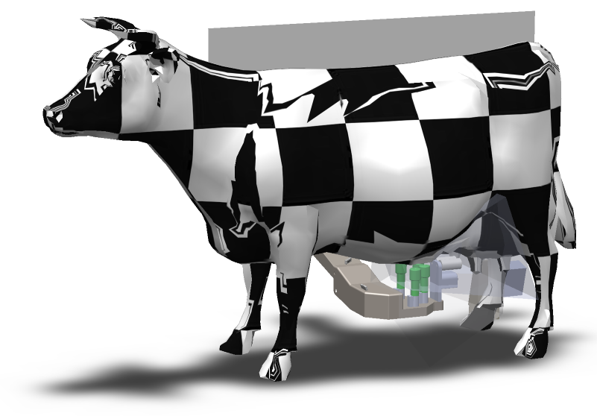
\includegraphics[width=0.65\textwidth]{images/cow_system.png}
        \caption{3D Prototype Model of the Cow Milking Robot}
        \label{fig:cow_fmc}
    \end{figure}
    
\section{Motivation}\label{chap:1:motivation}
% Use Case: Improving the Cow Milking Automation
It is believed that the first time a cow was milked was around 8,000-10,000 years ago, somewhere in Europe\cite{valente_2017}. Interestingly, milk also is given the credit for the developments that have happened in the modern food industry. Not only because of how widespread it is in today's culture, but also because of bringing cheese and butter with it. Over the past 8,000 years, more than a handful of technological advancements have happened, specially in the farming industry. The Agricultural Revolution proved to be a turning point for the food supply, allowing the way for the Industrial Revolution \cite{lumenlearning_2021}. Consequently, milking robots have been around in agriculture for over 20 years. However, the concepts of the widespread milking systems available on the market have hardly had any adaptations leveraging the latest technological advancements. The current largest supplier, Lely, still uses electro-pneumatic spindle motors even in the latest version of the milking robot (Astronaut A5). The benefit of these motors is their low cost and their physical compliance, making them resistant to cow kicks. They require, however, a lot of maintenance. For example, the seal of these motors must be replaced regularly so that the system remains operational. As of today, the herd size in Swiss farms is often big enough so that more than one milking robot would be needed, but the space requirements do not allow for this without having to remodel the barn's infrastructure.

A current project at the ZHAW aims to construct a milking robot that changes the current paradigm, in cooperation with the industrial partner Sutter Landtechnik GmbH (SLG). Most of today's milking robots use a 2D laser scanner to estimate the position of the cow, the udder and the cow's teats. During the position estimation, the robot is static and several measurements are necessary. This is time consuming and if the cow moves during the measurement, the position estimation must be reinitialized. The ZHAW proposes innovative changes to the milking robot's architecture, using electric drives and a more compact kinematic structure. Moreover given the inexpensive 3D cameras have been introduced to the market over the past few years, it is now possible to leverage of high resolution 3D point clouds to dynamically estimate the position of the cow teats.

Based on this background, the aim of this Vertiefungsarbeit (project work) is to select and implement a machine learning and computer vision enabled pipeline that estimates the 3D pose and direction of cow teats. The methods proposed in this work build the basic structure for an approach to estimate the position of the cow teats.

% Although this requires much more complex data processing on a powerful control system, it does away with a time-consuming, separate 
% time-consuming, separate measurement process can be dispensed with. Dynamic measurement with modern sensors also offers the potential to be much more robust and reliable than the measurement methods used today.
    
    % \begin{itemize}
    %     \item describe the general need for automated cow milking
    %     \item describe how the problem is currently being solved briefly
    
    %     \item describe the challenges in cow teat recognition: morphology/shapes and movement
    %     \item describe how these methods fail || describe challenges/limitations of current methods (sensors, etc, no memory)
    
    %     \item can solve this problem with computer vision briefly
    
    %     \item describe cow project main driver (The InIT's purpose) (do we mention how expensive current solutions are?)

    % \end{itemize}
% \section{The Need for Organic Milk}\label{chap:1:organic-milk}

% In recent years, the financial pressure on agriculture in Switzerland has increased massively. Since 1980, the number of farms has been shrinking by about 1000 farms per year. The Swiss consumer wants more and more organically grown products and at the same time consumer prices are getting cheaper and cheaper. The extensive Swiss animal welfare regulations, which are the strictest in Europe, make animal husbandry even more expensive. All this leads to the fact that the average income of a farmer family decreases annually. The farmers' association is therefore calling for greater support from the state. The SLG sees the key to running a profitable Swiss farm not in higher government subsidies, but in a more efficient machine park, which is specifically optimized for the Swiss market, according to Swiss legislation and for organic and ecological farming. All robotic milking equipment available today is not designed for organic farming but optimized to maximize milk yield. However, in the saturated Swiss milk market, what is needed is not more milk, but rather milk produced in a fair, organic and cost-efficient way.

% Across Europe, organically produced milk is still a niche product. However, the SLG is convinced that this will change in the coming years, as consumers in Europe are also paying more and more attention to what they eat and how their food was produced. The focus of a new development should therefore not be on maximizing the amount of milk per animal, but on minimizing investment and operating costs, and above all, these new systems should enable organic farming without compromise. This starts with giving cows access to pastures.

% Today's robotic systems are designed for 24/7 operation. Especially for smaller farms, this mode of operation is necessary to keep operating costs low. In contrast, an important feature of the new robotic system is to be able to milk all cows on a farm within one to two hours, thus combining all the advantages of a conventional milking parlor with the benefits of a milking robot. For this purpose, the new robot is dimensioned in such a way that several robot arms can be installed in the intermediate aisles of existing barns without the need for major cost-intensive building adaptations. By installing the robot in the intermediate aisles of the barn, it will also be possible to minimize the use of concentrated feed, as the cows will automatically pass the robot when moving from the cubicles to the feeding axles.

\section{Related Work}\label{chap:1:related-work}
As mentioned above, laser technology used in the current cow milking robots limits the performance of the systems, which can be improved by leveraging the latest technological advancements. As stated by \textcite{pal2017algorithm}, laser technology is not capable of differentiating between a cow's teat and a leg, therefore manipulating the suction cups in the wrong direction. Along these lines, \citeauthor{pal2017algorithm} propose a fast and reliable solution to the problem of 3D pose recognition of cow teats using TOF, RGBD and Thermal Imaging. 
% Their pipeline provides a new accurate way for estimating the poses but lacks any intelligence with respect to knowing what is a cow teat.
Similarly, \citeauthor{rastogi2019teat} take a stand against the limitations of laser assisted edge detection technologies, which cannot differentiate between a healthy and a diseased teat. They propose two alternatives to the task: a Haar-cascade classifier and a YOLO classifier for cow teats. Both approaches work on real time but lack reliable accuracy. The Haar cadcade classifier fails to detect any teats in the occluded tests, and YOLO fails to detect a fourth teat even with a prediction threshold of 0.5.
% Even though YOLO performs splendidly and even in real-time, YOLO provides only a bounding box for the object found, whereas a segmentation network benefits by separating the pixels of salient object from the background.
Additionally, \textcite{dorokhov2019recognition} analyzed the study from \textcite{akhloufi20143d} for vision systems for livestock and gathered that RGB-D technologies are preferable to ToF. Regardless, they propose a k-nearest neighbors approach from the point cloud captured by a ToF camera. They also state that the vacuum action in the teat attachment step allows for the teat pose estimation error to be at most 1 cm. They fail, however, to provide any benchmarks about the performance of their algorithm.

\textcite{ciocarlie2014towards} propose a complete software achitecture for reliable grasping of household objects. Their work combines scene interpretation from 3D data, grasp planning, motion planning and failure identification and recovery modules. Related to this work, their semantic perception approach uses Eucledian clustering on pre-segmented objects from a scene from a 3D point cloud. They then use a similar technique to the ICP algorithm to match the object clusters to a database of pre-defined 3D models. One of their main concerns for future improvements is that robots should be able to grasp objects in unknown scenarios.

On the same note, \textcite{manuelli2019kpam} state that manipulation policies should generalize to potentially unknown instances. Therefore, they introduce a novel category-level manipulation pipeline that uses semantic 3D keypoints for object representation and enables the specification for robot action planning and grasping with centimeter level precision. 

Finally, \textcite{o20193d} review 3D computer vision systems and techniques for precision dairy farming. More specifically, they look at Time of Flight and streoscopic vision systems. They conclude that robust systems which adapt to weather conditions, herd characteristics, farmyard layout, etc. (generally unknown scenarios) are required. Hence they foresee that the future state of the art technologies use Geometric Deep Learning for processing data in non-Eucledian domain, such as graphs and manifolds. \textcite{cao2020comprehensive} provide a comprehensive review of deep learning methods in the graph and manifold domain, including history, background, applications and benchmark datasets as reference for research in geometric deep learning.

On the similar final note, \textcite{arad2020development} propose an extensively tested and integrated system design for SWEEPER, a robot for harvesting sweet peper fruit in greenhouses. SWEEPER uses time-of-flight technologies and a single sensor for RGB and depth analysis, which combined with a shape and color-based detection algorithm allows high frame-rate operation. To summarize, they use they use traditional-computer-vision-enabled pipeline to analyze the morphology of the shapes recognized, and then compare its relative size to an average pepper size, which allows fast calculations. 
% , which is capable of autonomously driving on irregular floors. 


% 3D vision
\textcite{qi2018frustum} propose, after evaluating a new type of deep net architecture called PointNet\cite{qi2017pointnet}\cite{qi2017pointnet++}, a method that is able to localize objects in large-scene point clouds with high efficiency and high recall, regardless of heavy occlusion or with very sparse points. However their method struggles with multi-instance scenarios, pose estimation accuracy in sparse point clouds, and 3D detection if the 2D detector faces strong occlusion.

to obtain a point cloud of the cow teat  attempt to tackle the problem processing the point cloud 

% \section{Vision Systems in Automated Milking Robots}\label{chap:2:melkroboter}
% half a page

% Vision Systems in Automated Milking Robots

% The systems available on the market all consist of a manipulator and the associated basic equipment. Therefore, when using several manipulators at the same time, the basic equipment must also be present several times. The possibility of operating several manipulators on one base unit (the base unit contains the pumping and cooling units as well as the tanks for the milk) is not in itself a technical-scientific innovation. However, when several manipulators are used, the cost of the individual manipulator plays a significant role in the cost-effectiveness of the overall system. Therefore, the aim is to develop a manipulator that is cost-effective in terms of production, maintenance and operation, using state-of-the-art components. The content of this research project is limited only to the development of a new manipulator. The development of the complete system will be done by SLG outside this research project - the corresponding know-how is available due to years of experience in the development, production and maintenance of own milking systems. The in-house development of the overall system also allows SLG to determine all parameters of the milking process itself and thus adapt them to the specific conditions in Switzerland. The latter is not possible with the systems currently available.

% The robotic milking systems available on the market apply different strategies to detect the cows' teats. The goal is, after the cow has entered the milking parlor and the teats have been hygienically cleaned and stimulated, to apply the teat cups to the teats as quickly as possible. This involves moving the teat cup in front of the teat tip and then moving it in the direction of the teat towards the udder. Due to a vacuum, the teat cup then remains attached to the teat by itself until the vacuum is switched off after the milking process has been completed. Depending on the system, the cup is then removed by pulling back the hose hanging from the cup or by pulling on a separately attached rope.

% The attachment of the four buckets is done in the case of the Lely machines by moving a platform where all four buckets are moved simultaneously until they are attached. This design has the advantage that the
% This design has the advantage that the robot arm only has to travel the long way under the cow once per milking operation, and only short movements are then required for the attachment of the teat cups. In addition, if the cups do not stick to the teat, they fall back onto the platform and not onto the floor, where they become dirty and a time-consuming cleaning process becomes necessary. Thus, the docking time for these systems is typically about one minute for all four cups. However, this design also has drawbacks: The somewhat bulky design means that more volume must be moved between the cows' legs. This is uncomfortable for the cow and also means an increased risk of the cow stepping on or into the robot arm. In addition, the large mass of the platform also means that it is difficult to constantly follow the teat cups to the teat during the docking maneuver. Other products, such as DeLaval's VMS, use the robot to move each cup individually from a magazine next to the cow box to the teat. These manipulators can be built slimmer and lighter, allowing them to move more agilely. The disadvantage is that the docking process for four cups takes longer (about two minutes) and also that if the cup does not adhere properly to the teat, it will fall to the floor under the cow, requiring an additional cleaning procedure.

% The existing milking robots measure the position of the teats once before starting the docking procedure and then approach the teats in a purely position-controlled manner. In contrast, the new manipulator will be designed in such a way that it is able to detect the teats during the entire docking process in order to always be able to move the teat cup in the direction of the teat. This guarantees that even if the cow moves during the docking process, the teat is reached as quickly as possible and with a high degree of safety. In this way, the robustness and also the time of the docking process of the teat cups can be significantly improved. For this, in addition to the appropriate 3D sensor technology, a corresponding real-time evaluation algorithm is required. Furthermore, the manipulator itself must be designed in such a way that it can dynamically move a platform with the four teat cups accordingly. Last but not least, the control system must also be capable of executing sensor-guided movements in real time.

% Even if some competitors have equipped their latest milking robot models with more modern 3D sensors in the meantime, the sensor-guided dynamic target movement described here has not been implemented, among other things because the necessary manipulator design is not available.


\section{Purpose and Research Question}\label{chap:1:research-question}
In this work, a machine learning and computer vision based solution will be used to estimate the pose of cow teats for a milking robot. Regarding this task, this work tackles the following research question:
\begin{itemize}
    \item How can the cow teats 3D pose be estimated under 10 seconds?
\end{itemize}

\section{Approach and Methodology}\label{chap:1:approach-methodology}
This work focuses on computer vision techniques to manipulate RGB-D data to positions and directions of objects in 3D space. The problem that will be solved within this Vertiefungsarbeit is the pose estimation of cow teats.

The planned strategy for this project work is the following:

A state of the art analysis will be done to propose a processing pipeline that answers the research question. This analysis includes the evaluation of a variety of advancements computer vision and machine learning fields such as object segmentation, 3D object recognition, and pose estimation for the 3D pose estimation of cow teats. This also includes the implementations of the proposed algorithms and the respective optimization of their parameters to solve the task optimally. It is also important to note that this process has an iterative nature, where the validation of the models' results will trigger changes in the data sets and the diverse algorithms' parameters, in order to achieve the best possible results. The used data will be of both real and synthetic origins. Finally, the results will be critically evaluated and compared to each other. The reliability and limits of the results will be discussed and further improvements on this field will be considered. 


\section{Scope and Limitation}\label{chap:1:scope}
Due to the time constraints, some limitations have to be laid out to ensure the work can be finished within schedule.
\begin{itemize}
    \item The approach used will focus specifically on the manipulation of RGB-D images, while the manipulation of point clouds will be left out.
    \item This work focuses on the results observed in computer vision and machine learning approaches using 3D cameras. Other techniques, which for example use lasers for 3D scene understanding, will not be taken into account.
    \item This work does not take into account scene understanding and camera manipulation techniques.
    \item This work will focus on the 3D object recognition of cow teats for milking robots.
    % \item 
\end{itemize}
\section{Target Group}\label{chap:1:target-group}
First, this work of special interest for researchers in the field of computer vision. This is due to the fact that 3D object recognition is still a rapidly growing field.  Second, as mentioned in \ref{chap:1:motivation}, the industrial partner Sutter Landtechnik GmbH (SLG) is the private interest group for this research.  This is because SLG not only offers sales, installation and service of technical equipment and machinery for various tasks in agriculture, but also
% It is based in in Andwil and Muolen, Switzerland.
% Its customers are farms of various sizes in German-speaking Switzerland and in nearby foreign countries. 
provides milking technology, which includes milking robots of the "Astronaut" variant\cite{2021lely-a5}.
% , manufactured by the Dutch company Lely. 


% In addition to the areas of tractors and agricultural technology (e.g. harvesting machines), farm technology (barn equipment), there is the area of milking technology, which, in addition to milking machines, includes cooling technology and, last but not least, milking robots. 

% Various machines, including milking technology, were developed by SLG itself and are also manufactured in its own plant. Of the approximately 50,000 farms in Switzerland, about 2,000 are customers of SLG. In addition, there are about 200 farms from nearby foreign countries. With these, SLG generates an annual turnover of ~6.3 MCHF (2018) with its 25 employees. All milking robot systems installed and/or maintained by SLG are of the "Astronaut" type from the Dutch company Lely.

% As the Lely company was not interested in product adaptations for the Swiss market, SLG terminated its direct business relationship with Lely in 2016 and decided to develop its own robotic system. Therefore, in this project, the prototype of a low-cost, modern milking robot suitable for the specific Swiss requirements will be developed, which can be manufactured and marketed by Sutter Landtechnik GmbH (SLG) itself.

% The Lely company with the Astronaut model range has been able to establish itself on the European market for a variety of reasons and is by far the market leader. The European market is dominated by two brands, Lely 55\% and DeLaval 30\% of the market. In Switzerland there are currently around 850 Lely Astronaut and around 300 DeLaval VMS milking robots in operation. The Swiss market is clearly dominated by Lely with a market share of about 72\%. The weak competition, as well as the small Swiss market in relation to Europe, means that specific adaptations only for the Swiss market are not worthwhile for the large groups.
\section{Outline}\label{chap:1:outline}
The following Chapter 2 will cover the theoretical background for this work, making emphasis on computer vision, machine learning approaches, 3D object recognition, and pose estimation. Chapter 3 will describe the methodology, the nature of the data and the pose estimation pipeline's architecture. Chapter 4 will present the achieved results, and chapter 5 will examine the validity and reliability of the presented results. Finally, chapter 6 provides a conclusion and proposes further steps on research for this topic.
% \section{Towards 3D Object Detection}\label{chap:1:detection}

% \lipsum[2-5]

    % \begin{itemize}
    %     \item describe advancements in traditional computer vision for image interpretation
    %     \item list shortcomings/challenges we can overcome with computer vision
        
    %     \item describe advancements in computer vision with DL for object detection
    %     \item list shortcomings/challenges we can overcome with computer vision
        
    %     \item shortcoming1: no object permanence | objects out of sight
    %     \item shortcoming2: reliability of only detecting cow teats (?)
    %     \item HELP: shortcoming3: (?) (need to re-read the papers from gio)

    % \end{itemize}
% \section{Problem Description}\label{chap:1:problem}
% \lipsum[2-3]





% Als Resultat dieses Forschungsprojekts steht der Prototyp eines modernen Melkroboters, welcher durch seine auf kleinere Betriebe angepasste Konstruktion und aufgrund der eigenen Produktion und dem direkten Vertrieb durch SLG auch in kleineren Landwirtschaftsbetrieben rentabel eingesetzt werden kann. Die Forschungsresultate sind für SLG einfach und zeitnah in ein Produkt umwandelbar, welches direkt im Schweizer Landwirtschaftsumfeld vermarktet werden kann und somit im Bereich Landwirtschaft zu einer besseren, effizienteren und ökologischeren Produktion beitragen wird.

    % \begin{itemize}
        % \item in this work we answer the question: ---
        % \item we start by describing:
        %     \SubItem state of algorithms for cow milking
        %     \SubItem state of algorithms for 3d object detection
        %     \SubItem describe the system is able to localize cow teats in 3d space
        %     \SubItem describe the diverse algorithms we evaluated and tested (?)
        %     \SubItem finally we discuss the outcome of experiments and how to interpret conclusions
        %     \SubItem REWRITE/REUSE THIS SENTENCE FROM THESIS: We do not attempt to solve the specific use case of the ZHAW Summit XL Steel mobile robot, but aim to create an approach which is helpful in a large range of possible scenarios, similar to the way 3D mapping systems already enable robotic interaction today.
    % \end{itemize}

\chapter{Related Work}\label{chap:background}
% \section{Background and Related Work}
% 3 pages max, i was expecting 


\section{Traditional Object Segmentation Systems}\label{chap:2:segment}
% \lipsum[2-5]

With the rise of CNNs, the foundation has been set for well-performing image classification approaches such as ResNet [6] or VGG [7]. In recent years, this development has gone even further towards systems which are capable of localizing or even masking out objects in images. Popular approaches with these capabilities are for example Mask R-CNN [9] or YOLO [8]. While using different approaches, both systems have the capability of localizing and semantically classifying objects in images. Mask R-CNN is even able to mask the pixel-areas that are belonging to the object by using polygonal shapes. In the background both approaches still rely on ResNet for feature extraction.

While systems like these are highly impressive and sufficient for many cases, they are still far away from human visual perception and actual scene understanding [10]. Especially the shortcomings presented in section 1.2 apply to this kind of systems. The resulting polygon-masks or bounding boxes are not projected into 3D space but merely mapped onto the 2D coordinates of the image. If employed on sequential data, both systems would also need to reevaluate the whole frame on each timestep as they are not able to remember or track objects. This is problematic when understanding a scene, as it is often not likely for the whole scene to be visible at once, but only partially. Therefore we believe, it is crucial for a system not to forget but to accumulate information over timesteps.

Object detection is a computer vision task that attempts to localize and classify objects within an image. An extension of the problem involves assigning labels to the specific pixels in the image that belong to the detected objects, instead of only using the bounding boxes obtained during localization (object segmentation). 

Research on object segmentation built upon previous models to reach the current state of the art of 2D object detection, which is called Mask R-CNN. The image saliency approach each (previous) model takes is described below:
\begin{itemize}
    \item \textbf{R-CNN:} a “selective search” algorithm proposes bounding boxes and features are obtained using a deep convolutional neural network (for example, AlexNet). Object classifications are then made with linear SVMs.
    \item \textbf{Fast R-CNN:} unifies the feature detector, and the bounding box predictor approach into a single model, but the region of interests are still part of the input. The shared computation showed speed improvements.
    \item \textbf{Faster R-CNN:} unifies the region proposal algorithm into the CNN model. This model merges a RPN (region proposal network) with Fast R-CNN.
    \item \textbf{Mask R-CNN:} extends the previous model to add pixel-level image segmentation. A small fully connected network was added that per region of interest outputs a segmentation mask.
\end{itemize}


% %  half a page
%     \begin{itemize}
%         \item one paragraph of ML advancements 1960 - 2010
%         \item one paragraph how these methods are good at image processing but they showed lack of reliability without actually understanding what is in the scene
%     \end{itemize}
\section{Going into the 3D World}\label{chap:2:3d}
%  half a page
\lipsum[2-5]

    % \begin{itemize}
    %     \item one paragraph of rise of CNNs 2010 - present
    %     \item one paragraph how these methods are not enough for 3d space yet, and importance of not forgetting over timesteps
    % \end{itemize}
\section{Automated Milking Robots}\label{chap:2:melkroboter}
% half a page
The systems available on the market all consist of a manipulator and the associated basic equipment. Therefore, when using several manipulators at the same time, the basic equipment must also be present several times. The possibility of operating several manipulators on one base unit (the base unit contains the pumping and cooling units as well as the tanks for the milk) is not in itself a technical-scientific innovation. However, when several manipulators are used, the cost of the individual manipulator plays a significant role in the cost-effectiveness of the overall system. Therefore, the aim is to develop a manipulator that is cost-effective in terms of production, maintenance and operation, using state-of-the-art components. The content of this research project is limited only to the development of a new manipulator. The development of the complete system will be done by SLG outside this research project - the corresponding know-how is available due to years of experience in the development, production and maintenance of own milking systems. The in-house development of the overall system also allows SLG to determine all parameters of the milking process itself and thus adapt them to the specific conditions in Switzerland. The latter is not possible with the systems currently available.

The robotic milking systems available on the market apply different strategies to detect the cows' teats. The goal is, after the cow has entered the milking parlor and the teats have been hygienically cleaned and stimulated, to apply the teat cups to the teats as quickly as possible. This involves moving the teat cup in front of the teat tip and then moving it in the direction of the teat towards the udder. Due to a vacuum, the teat cup then remains attached to the teat by itself until the vacuum is switched off after the milking process has been completed. Depending on the system, the cup is then removed by pulling back the hose hanging from the cup or by pulling on a separately attached rope.

The attachment of the four buckets is done in the case of the Lely machines by moving a platform where all four buckets are moved simultaneously until they are attached. This design has the advantage that the
This design has the advantage that the robot arm only has to travel the long way under the cow once per milking operation, and only short movements are then required for the attachment of the teat cups. In addition, if the cups do not stick to the teat, they fall back onto the platform and not onto the floor, where they become dirty and a time-consuming cleaning process becomes necessary. Thus, the docking time for these systems is typically about one minute for all four cups. However, this design also has drawbacks: The somewhat bulky design means that more volume must be moved between the cows' legs. This is uncomfortable for the cow and also means an increased risk of the cow stepping on or into the robot arm. In addition, the large mass of the platform also means that it is difficult to constantly follow the teat cups to the teat during the docking maneuver. Other products, such as DeLaval's VMS, use the robot to move each cup individually from a magazine next to the cow box to the teat. These manipulators can be built slimmer and lighter, allowing them to move more agilely. The disadvantage is that the docking process for four cups takes longer (about two minutes) and also that if the cup does not adhere properly to the teat, it will fall to the floor under the cow, requiring an additional cleaning procedure.

The existing milking robots measure the position of the teats once before starting the docking procedure and then approach the teats in a purely position-controlled manner. In contrast, the new manipulator will be designed in such a way that it is able to detect the teats during the entire docking process in order to always be able to move the teat cup in the direction of the teat. This guarantees that even if the cow moves during the docking process, the teat is reached as quickly as possible and with a high degree of safety. In this way, the robustness and also the time of the docking process of the teat cups can be significantly improved. For this, in addition to the appropriate 3D sensor technology, a corresponding real-time evaluation algorithm is required. Furthermore, the manipulator itself must be designed in such a way that it can dynamically move a platform with the four teat cups accordingly. Last but not least, the control system must also be capable of executing sensor-guided movements in real time.

Even if some competitors have equipped their latest milking robot models with more modern 3D sensors in the meantime, the sensor-guided dynamic target movement described here has not been implemented, among other things because the necessary manipulator design is not available.


    % \begin{itemize}
    %     \item one paragraph about cow robot milking industry
    %     \item ??
    %     \item one paragraph about cow teat morphology 
    % \end{itemize}
\section{Summary}\label{chap:2:summary}
% half a page
\lipsum[2-5]

    % \begin{itemize}
    %     \item one paragraph: describe popular approaches briefly, and main ways literature does it
    %     \item 1P: highlight most interesting literature approach
    %     \item 1P: lastly, we discuss how X is done, and whether it is feasible to extend our approach (prob a small filler?)
    % \end{itemize}

\chapter{Method}\label{chap:design}
\begin{figure}[!ht]
        \centering
        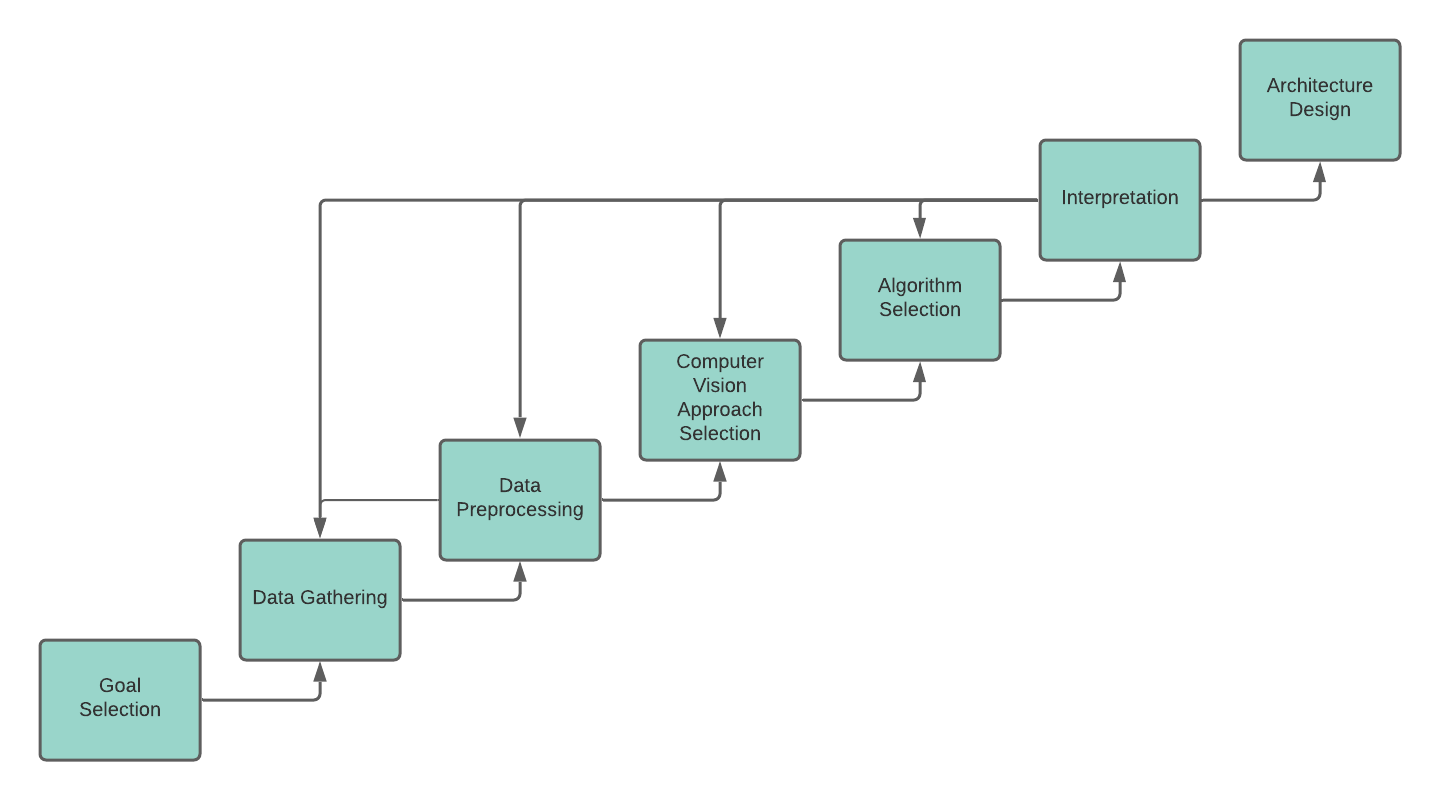
\includegraphics[width=1\textwidth]{images/adapted_development_process.png}
        \caption{Adapted development process from "\citetitle{luckert2016using}", by \textcite{luckert2016using}. Describes the taken steps from data collection, through algorithm selection to architecture design.}
        \label{fig:development_design}
\end{figure}
In this chapter the different steps taken to create a 3D object detector are addressed. 
This chapter adapts the structure proposed for machine learning algorithms proposed by \textcite{luckert2016using}.
The following questions are answered over the course of this chapter:
\begin{itemize}
    \item How can cow teats be recognized?
    \item What are the current method's goals and limits?
    \item What is the method's pipeline composed of?
    \item What is required to apply the method?
\end{itemize}


In order to answer these questions, the structure of this chapter is illustrated as follows: Section \ref{chap:3:goal} describes the first step. It defines the computer vision task and limits its scope. Then, the choice of a suitable data set and the composition of the collected raw data is presented. Section \ref{chap:3:data} describes the information available and the choice of features for the given task. Afterwards, it describes the preprocessing of the data by identifying noise or erroneous inputs. Section \ref{chap:3:method} describes the choice of three proposed processing pipelines and the considered algorithms and techniques.  The interpretation of the performance of the algorithm is described in Section \ref{chap:3:interpretation}. This section also describes how the method results were evaluated, how the algorithms were compared to each other and which parameters were adjusted. Finally, Section \ref{chap:3:architecture} describes the architecture of the processing pipeline, illustrating the diverse components' behaviors, interactions and deployment constraints.
% dacross for determining the 3D position of the salient object. 
% It also sets out the assumptions we took and the choices of technologies with respect to what was discussed in Section 2.

% domain model
%  
\section{Identification of the Computer Vision Goal}\label{chap:3:goal}
The predetermined goal of this project work was to propose a 3D object detection of cow teats solution using machine learning. As mentioned in Section \ref{chap:1:problem}, this project work tackles the following research question: 
\begin{itemize}
    \item How can the cow teats 3D pose be estimated under 10 seconds?
    % \item How can the cow teats 3D pose and direction estimation be evaluated?
\end{itemize}
To answer this question, the following practical steps were laid out:
\begin{itemize}
    \item Conceive a computer vision processing pipeline with optimal prediction quality for identifying the 3D pose and direction of a cow teat.
    \item Present a method for evaluating the quality of the predictions regardless of the method used.
\end{itemize}
This strategy was determined because the steps for data creation and preprocessing are independent of the approach used. Therefore, the remaining task is to propose a machine-learning-enabled pipeline that solves the indicated computer vision task without a priori knowledge of the input system. The main challenge in the processing pipeline is the usage of the diverse types of information the input system provides. The method for evaluating the quality of the predictions will then be built on the results of the processing pipeline. Therefore, the computer vision task is solved by the first step and and the second one is solved by looking at the prediction outputs.

\section{Image Data}\label{chap:3:data}
In order to evaluate computer vision predictions it is essential to gather sufficient quantities of raw data and to layout a simple data structure as required. The following questions will be answered in this section:
\begin{itemize}
    \item What kind of data is necessary?
    \item What kind of structure fulfills the requirements for the present study?
    \item What is the origin of the data?
    \item What are the preprocessing steps?
\end{itemize}
Traditional computer vision tasks require the following types of data: a training data set, for training the algorithm on the domain-specific data and a test set to determine the algorithm's prediction quality. As stated in Section \ref{chap:3:goal}, the given task is to estimate the 3D pose and direction cow teats for a cow milking robot. Therefore, the input data current accessible is: an RGB image, a depth image and a point cloud. The first attempts at tackling the problem using depth images for object classification using traditional computer vision methods failed to meet the performance criteria. Also, under the current project's conditions it is not viable to manually annotate a point cloud. It is also unfeasible to load a batch of point clouds into memory for training. Given the lack of additional inputs, each entry of the data set contains:
% to show any prediction outputs, and the execution time was over 300ms
\begin{itemize}
    \item RGB image of the cow teats.
    \item Pixel-wise segmentation mask, labeling the locations of the cow teats in the RGB image.
\end{itemize}
The nature of the data was two fold: synthetic and realistic. The collection of the realistic data was done at a laboratory at the ZHAW. Given the limitations of the first iteration of the milking robot project, the collection of real cow images was not required. The environment setup and details of the training data collection are described in Chapter \ref{chap:evaluation}. Finally, even though the images collected from the camera could be directly used for training, the preprocessing required was the adaptation of the data set to the COCO data format. Once formatted, the neural network could be trained.

Consequently, the collection of the synthetic data was done using Unreal Engine 4 and a plugin from NVIDIA \cite{2021ue4} called NDDS \cite{2021ndds}. Photorealistic scenes are created in Unreal Engine 4 and NDDS allows for the annotation of objects in UE4. These scenes are then exported and all the information from the objects is included in the export, such as objects, classes and 3D poses. Additionally, the export includes the respective rgb image, depth image, instance segmentations and class segmentations for the frame taken. Appendix \ref{appendix:ndds} illustrates a 3D scene and an export sample.

\section{Specification of a Computer Vision Approach}\label{chap:3:method}

This section describes choice of a computer vision approach for object segmentation, the proposal of 3d pose estimation pipelines and the actual processing step. The following questions will be answered in this section:
\begin{itemize}
    \item Which and how many approaches were considered appropriate for the object segmentation task?
    \item Which and how many approaches were considered appropriate for the pose estimation task?
    \item What optimization steps were taken on the algorithm for the data set?
    \item What were the main problems found during this phase?
\end{itemize}
A trade-off between machine learning techniques is always involved when comparing the advantages and disadvantages of each approach. Therefore, a variety of approaches were considered for the mentioned tasks, evaluated and optimized.

\subsection{Object Segmentation Approaches}

As described in Section \ref{chap:2:segment}, object segmentation involves the pixel-wise assignment of labels in an image that belong to a specific class. The following techniques were considered suitable for this task:
\begin{itemize}
    \item \textbf{Thresholding} A threshold value divides the pixels by intensity value, into background and foreground, generating a binary image.
    \item \textbf{K-Means clustering} A K number of clusters is given to divide the data in to K groups or clusters, based on similarity.
    \item \textbf{Histogram-based image segmentation} A histogram is used to group pixels based on gray levels, where the background is one big peak and then the other "hills" are objects.
    \item \textbf{Edge detection} Changes in brightness are identified using filters to locate edges, curves and shapes. 
    \item \textbf{Convolutional Neural Networks} As described in Section \ref{chap:2:segment}, convolutional operations are used to label the pixels. This approach scans the image by segments, for example using a sliding windows approach.
    \item \textbf{Fully Convolutional Networks} Contrary to to CNNs, FCNs can take different kinds of input, and output a matrix of dimensions H x W x C (image height, image width, number of classes).  
\end{itemize}
Among all the suitable methods tested, the segmentation problem was best tackled using two implementations of MaskRCNN: matterport/MaskRCNN and Detectron2 (FacebookAI). The evaluation and performance of both approaches is described in Section 5.

%As of 28.12.2020, MaskRCNN's repository has not been updated since 01.04.2019 and has over 1500 issues.

\subsection{Pose Estimation Approaches}

As described in Section \ref{chap:2:segment}, object segmentation involves the pixel-wise assignment of labels in an image that belong to a specific class. The following techniques were considered suitable for this task:
\begin{itemize}
    \item \textbf{Recognition of Fixed Shapes} A set of features are generated from the geometric information, such as 3D points, lines or surfaces. These features are then matched to a predefined model features. If the similarity evaluation between the model and the detected features is sufficient, a frame transformation is executed to identify the pose of the detected object. This pose detection represents a hypothesis, among many other hypothesis which are generated while evaluating, for example, a point cloud. Therefore, an appropriate criteria must be used to determine if the hypothesis should be accepted or rejected (hypothesis evaluation). An alternative approach consists of single generating descriptor features from clusters generated in a scene for posterior matching.
    \begin{description}
    \item \textbf{Algorithm Used: } RANSAC \cite{2021scikit-ransac}.
    \end{description}
    
    \item \textbf{Recognition of Object Classes} An algorithm is used to recover a 3D model from the input (image or point cloud), which is then segmented and then classified. Methods like an RDF classifier or CNNs can be used for classification. Then, methods like surface-to-surface distance minimization are used to retrieve the best match. Both realistic and synthetic RGB-D data sets have been published over the past few years for training and testing RGB-D algorithms. Furthermore, it is important that these methods are able to infer the complete 3D shape from a single frame, specially for robotic tasks like grasping.
    \begin{description}
    \item \textbf{Algorithm Used: } DOPE \cite{tremblay2018deep}.
    % \item \textbf{Algorithm Used: } 

    \end{description}
    
    \item \textbf{Feature-based Recognition} Similarly to the recognition of fixed shapes, a set of 3D descriptor features are generated from the geometric information (keypoints) and then evaluated. These descriptor features can be defined by a set of  parameters, such as point coordinates unit vector orientations, point feature histograms of the local surface properties (PFH), etc. A major advantage of these methods is that they require only a single correct feature correspondence to recognize an object.
    \begin{description}
    \item \textbf{Algorithm Used: } Manual Manipulation "MAV". This algorithm leverages the segmentation mask and overlays it over the depth image. Afterwards, the 2D points are proyected into 3D space and PCA is used to calculate the teat direction. Finally, the N points (averaging method) at the bottom of the teat (using the direction indicated by PCA's first component) are averaged to obtain a "teat's tip coordinates". A manual offset was added to the obtained coordinates to attempt to fix the (x,y,z) error observed.
    \end{description}
    
\end{itemize}
\begin{figure}[!ht]
        \centering
        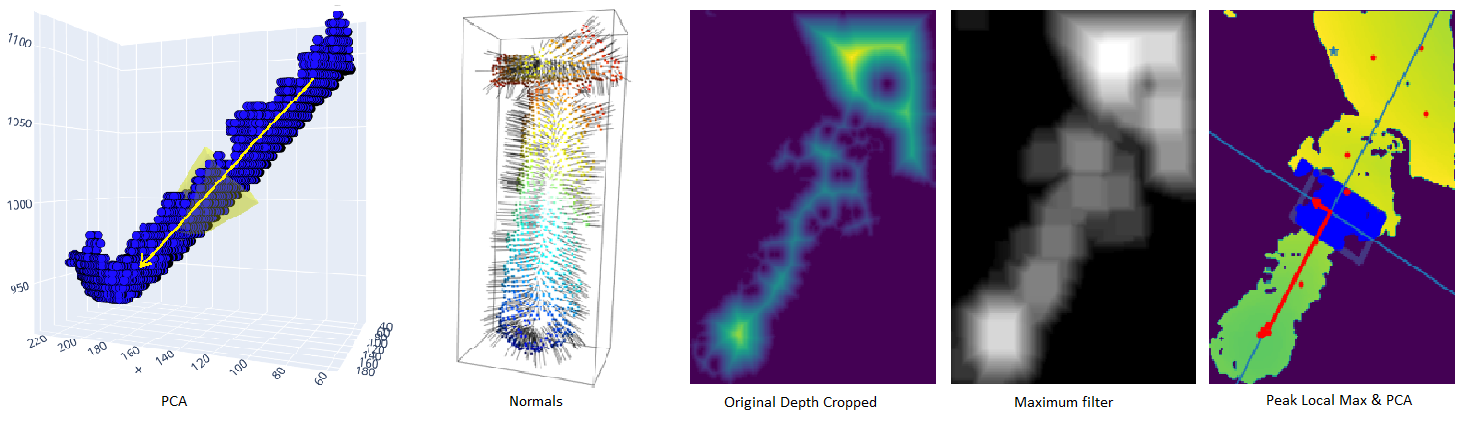
\includegraphics[width=0.8\textwidth]{images/cow_pose_methods.png}
        \caption{Illustration of algorithms to analyze 2D and 3D features. From left to right: PCA in a 3D scatter plot; normals of the points found; 2D erosion to remove outliers, dilation and usage of PCA to find points direction.}
        \label{fig:cow_fmc}
    \end{figure}
For each of the methods described above implementations were chosen to predict based on the data sets.  It is important, during the construction and training of a classifier, to tune the parameters of each model. On one hand, for the object segmentation approach, the parameters that were tuned were the learning rate, the score threshold for prediction, the number of workers, the number of iterations, the images per batch and the batch size. On the other hand, for the pose estimation approaches many parameters were tuned, specific to the method, such as maximum number of cow teats in memory, memory tracking reset conditions, frame transformations, etc.

There were several challenges faced during this phase. Both synthetic and realistic data sets were used for validating not only the models but also the data sets. It was observed that 1) some implementations of the segmentation network used were slower than the final implementation used and 2) the synthetic data set was too different and the reality gap could not be closed. Additionally, allocating resources in the CPU posed a problem in the diverse training and testing. This could be solved by allocating resources in a remote GPU cluster, but set different kind of limitations in the development process.  Finally, due to the fact that many algorithms were tested, the architecture's base concept was a modular design with a plug-and-play approach.

\section{Interpretation}\label{chap:3:interpretation}
%  This section also describes how the method results were evaluated, how the algorithmswere compared to each other and which parameters were adjusted
In order to determine, which implementation of the algorithms work best, a set of metrics need to be taken into consideration to evaluate the outputs of the different algorithms. The metrics are described in Chapter \ref{chap:evaluation} and were used to adjust the data sets and tune both the training and prediction parameters of the algorithms. In the current task there is only one label, so the label distribution is not a challenge. Therefore, a low misclassification rate or respectively a high accuracy rate can be treated as an algorithm result of very high quality \cite{luckert2016using}. On one side, to improve the segmentation algorithm's accuracy, both false positives and false negatives were identified, labelled and added to the data set. On the other side, to improve the pose algorithm's accuracy, different approaches were taken. For example, in the MAV algorithm an offset was calculated and added manually, and an averaging mechanism was added to calculate the cow teat's tip. Subsequently, a correlogram was used to analyze the influence of the camera position and orientation on the error estimation. The correlation coefficients proved a strong indirect correlation and the error showed to be normally distributed. Therefore, linear models are a promising step for predicting and subtracting the error. 
% It is part of the further steps in Chapter \ref{chap:conclusion} to minimize the error offset using a separate algorithm. 
To compare the algorithms among each other, the average error from the errors in (x,y,z) against the cow teat's tip ground truth was evaluated. 

\section{Processing Pipeline}\label{chap:3:architecture}
\begin{figure}[!ht]
        \centering
        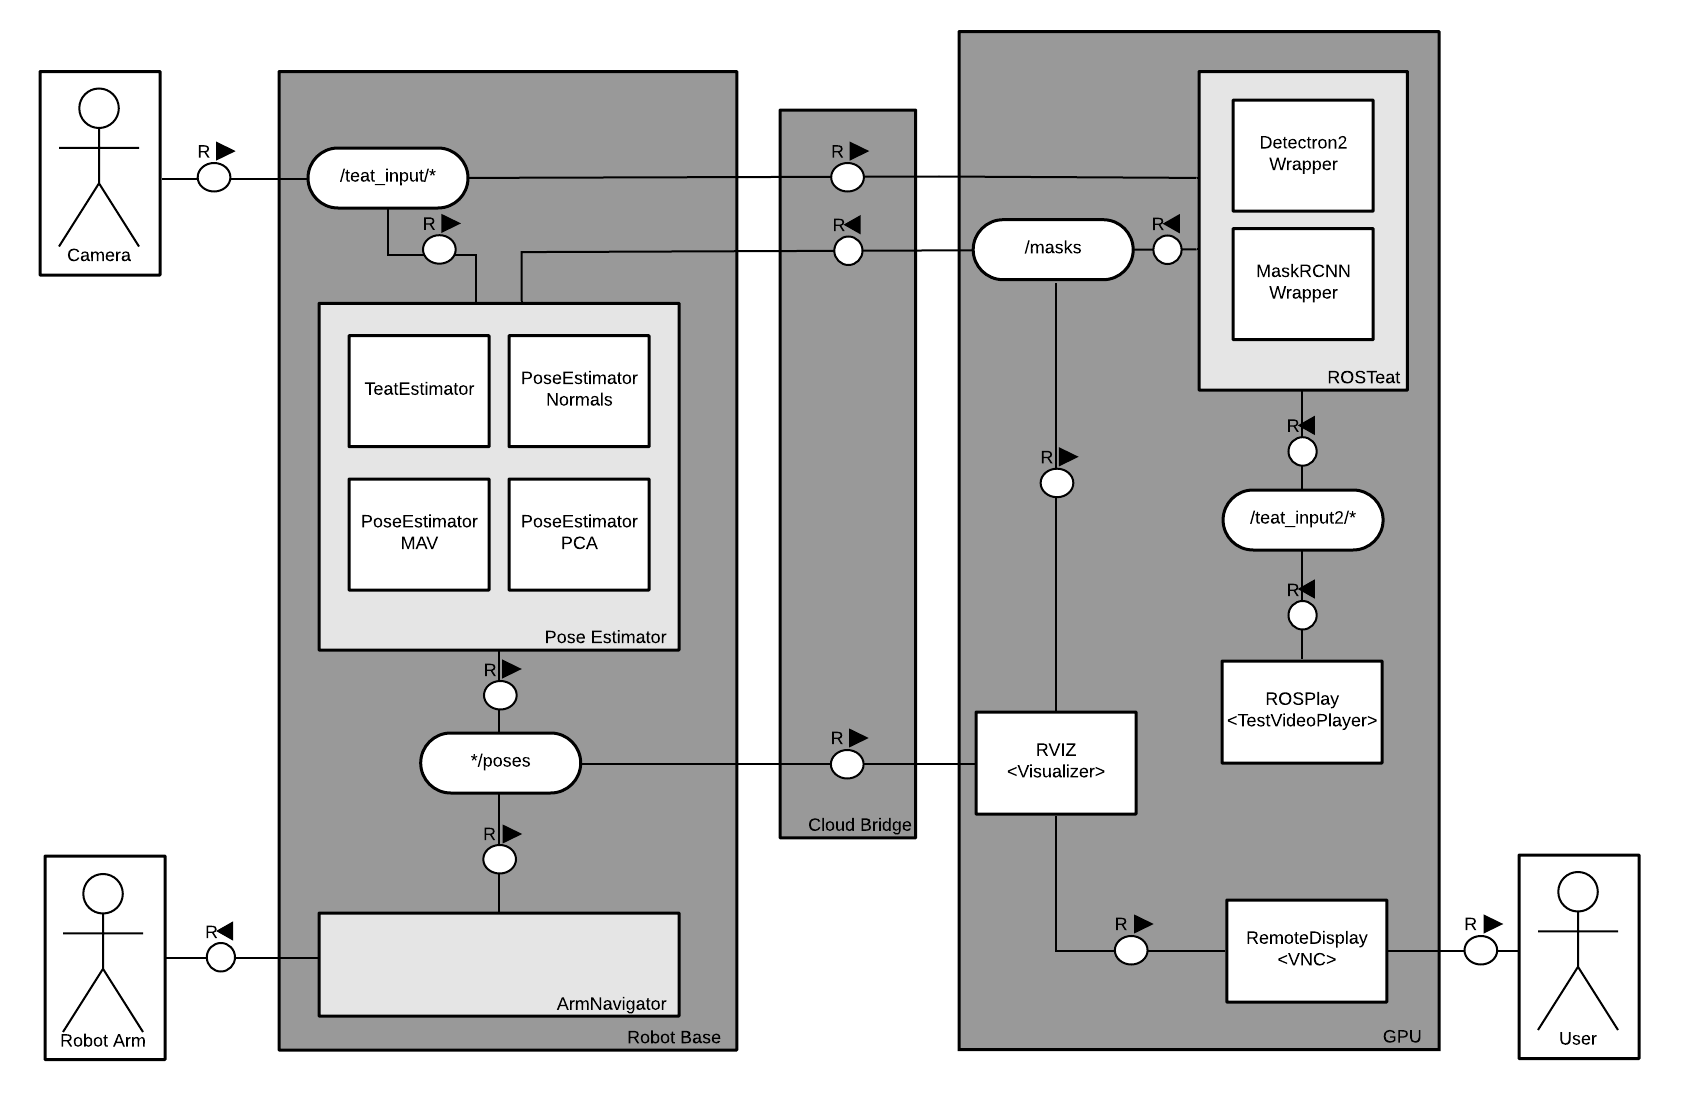
\includegraphics[width=.9\textwidth]{images/cow_fmc.png}
        \caption{FMC diagram of the Pipeline's Architecture}
        \label{fig:cow_fmc}
    \end{figure}
% \section{Software Design} 
% \section{FMC Diagram}
As a tool for designing a modular architecture, a domain model is used to help solve and understand the complexity in the system. The Fundamental Modeling Concepts (FMC) provide a framework for the comprehensive description of software-intensive systems \cite{FMCdiag}. 
% Its block diagrams show the compositional structures as a composition of collaborating system components.
In this framework, active system components are called agents and passive system components are called locations (storage, channels, queues; where information can be observed). The FMC diagram in Figure \ref{fig:cow_fmc} describes the high-level overview of the system's architecture, which illustrates the following agents and locations:
\begin{itemize}
    \item \textbf{Camera:} captures frames and publishes these as input for all the other components.
    \item \textbf{User:} uses Rviz to visualize: the point cloud, the RGB image, the depth image, the segmented image of the cow teats and the 3D poses published.
    \item \textbf{Robot Arm:} moves according to the instructions given by ArmNavigator. 
    \item \textbf{PoseEstimator:} pose estimation algorithm that processes the information received from the camera and ROSTeat to predict 3D poses.
    \item \textbf{ROSTeat Node:} processes images from the Camera node and segments the cow teats in the image.
    \item \textbf{ArmNavigator:} manipulates the RobotArm according to the 3D poses published.
    \item \textbf{ROSPlay <TestVideoPlayer> Node:} Behaves as a simulation/testing mechanism for reproducing the camera videos.
    \item \textbf{RVIZ <Visualizer>:} ROS framework that allows the visualization of different ROS topics (RGB image, point cloud, etc.)
    \item \textbf{RemoteDisplay <VNC>:} this is a browser-based graphical-d
    esktop system that allows the visualization of RVIZ.
    \item \textbf{/teat input/*:} channel where the camera input is published for other components to consume.
    \item \textbf{/teat input2/*:} channel where the simulation video is published as input for other components to consume.
    \item \textbf{/masks:} channel where the segmented cow teats are published.
    \item \textbf{*/poses:} channel wehre the 3D cow teat poses are published.
\end{itemize}
One of the problems that appeared during this phase, was communicating the ROS (Robot Operating System) published messages across two networks. 
% The ROS topics are the buses over which ROS nodes exchange messages (input images, masks, poses, etc.)\cite{2020ROStopics}.
After thorough research it was found that ROS needs a routing mechanism that forwards the published topics (communication buses) from the Robot Base to the GPU and vice versa. The Cloud Bridge uses agents which are deployed on each network, to allow the intercommunication of topic messages. This allowed the deployment of the segmentation network in the GPU cluster, and the pose-estimation-related components in the Robot Base. 
% The behavior and interactions of the main components (ROSTeat and Pose Estimator) are described in the following sections with more detail.

\subsection{Use Cases}
As part of the analysis process, one of the well established fundamental techniques is used: use cases. The use cases identified, which capture the black box requirements requirements for the given task, are 1) cow teat segmentation and 2) pose estimation. The sequence of activities and events described Table \ref{tab:use-segment} and Table \ref{tab:use-pose} takes special conditions and exceptions into consideration.

\begin{longtable}{@{} p{3.5cm} p{10.5cm} @{}} \toprule
\textbf{Use Case}       & \textbf{Segment Cow Teats from Image} \\ \midrule
Actor                   & ROSTeat Node \\ \cmidrule{1-2}
Description             & A cow teat is recognized from an image. \\ \cmidrule{1-2}
Goal                    & Publish the cow teat masks present in received image. \\ \cmidrule{1-2}
Preconditions           & An image exists. \\ 
                        & ROSTeat node is running. \\ \cmidrule{1-2} 
Postconditions          & A number of masks have been identified from image [0+]\\ \cmidrule{1-2} 
                        & 1. The camera publishes an image. \\ 
Basic Flow              & 2. The ROSTeat node consumes the image and predicts the cow teats in it. \\
                        & 3. The ROSTeat node publishes the masks for future processing. \\ \cmidrule{1-2}
Exceptions             & Image is not RGB \\ \bottomrule
\caption{Use Case - Predict Masks} \label{tab:use-segment} \\
\end{longtable}

% \newpage
\begin{longtable}{@{} p{3.5cm} p{10.5cm} @{}} \toprule
\textbf{Use Case}       & \textbf{Estimate 3D Pose of Cow Teat} \\ \midrule
Actor                   & Pose Estimator \\ \cmidrule{1-2}
Description             & A cow teat pose is recognized from a tuple (image, point cloud, depth image, mask). \\ \cmidrule{1-2}
Goal                    & Publish the cow teat poses for each message received. \\ \cmidrule{1-2}
Preconditions           & An image exists. \\ 
                        & ROSTeat node is running. \\ \cmidrule{1-2} 
Postconditions          & A number of cow teat poses have been identified from image [0+]\\ \cmidrule{1-2} 
                        & 1. The camera publishes an image AND ROSTeat node publishes the masks for the image (synchronized receival, stored as a tuple). \\ 
Basic Flow              & 2. The Pose Estimator node consumes the tuple and predicts the cow teat poses in it. \\
                        & 3. The Pose Estimator node publishes the poses for posterior attachment. \\ \cmidrule{1-2}
                        \\
                        \cmidrule{1-2}
Exceptions             & TransformListener is empty \\ 
                       & Any element in the tuple is empty and masks are not (data corruption). \\ \bottomrule
\caption{Use Case - Predict Poses} \label{tab:use-pose} \\
\end{longtable}

\subsection{Design}
Given the nature of the recognition problem, it was determined that it is important to minimize assumptions on poses or camera angles (frame information) and account for the natural variation of the cow teats (udder morphology, colors, light conditions, etc.) as described in Section \ref{chap:2:melkroboter}.
Figure \ref{fig:cow_topics} aids to illustrate a high-level overview of the communication fashion between components.
Finally, given the modular design and message-based principles laid out, allowing any pose estimation algorithm to be used, the pipeline's proposed design is described below:

\begin{enumerate}
    \item The camera publishes information (RGB image, point cloud, depth image) into the input ROS topic channel, which is consumed to identify the position and size of salient objects.
    \item The ROSTeat node subscribes to this input channel, uses the neural network to predict the cow teat masks and publishes them into a masks channel.
    \item The Pose Estimator (plug-and-play component) consumes the masks that were published, and synchronizes it with the camera information (so it is all processed as a single message). The following pose estimation is algorithm-specific. Each pose estimation algorithm is described in detail in the following section. The poses are then published into a poses channel.
    \item The robot consumes messages from the poses channel and moves 10-15 cm forward towards the indicated 3D poses, until it is 20-30 cm close to the pose estimations. Then the attachment process is initiated.
\end{enumerate}

\begin{figure}[!ht]
    \centering
    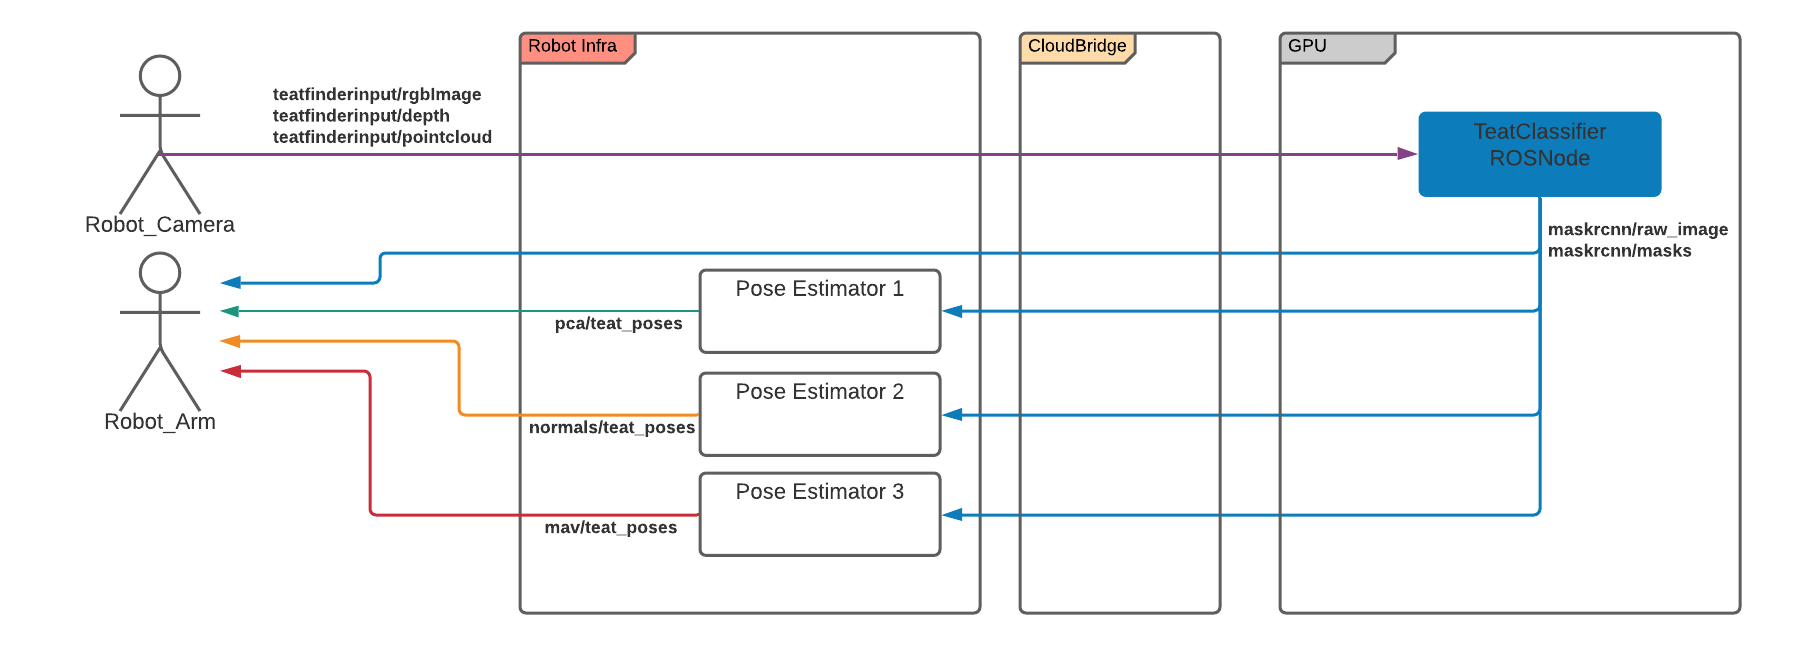
\includegraphics[width=1\textwidth]{images/cow_topics.png}
    \caption{High-level flow diagram of the teat estimation pipeline.}
    \label{fig:cow_topics}
\end{figure}

%  As explained in Section \ref{chap:3:architecture} the messages must go through a Cloud Bridge to be able to connect the robot's ROS local topics with the GPU ROS topics. 


As described above, the interactions between the camera and the recognition components depend on the messages received (images, masks). In order to improve the efficiency of the development process, the ROSPlay component was introduced to allow the repetition of camera frames from a ROSbag (ROS format for a video file). A ROSBag is then used for data generation, algorithm training and testing. One of the problems encountered in this phase was that the generated ROSbags are up to 20 GB in size. These ROSBags are generated in the ROS Base and have to be transferred over the network to the development environment (local laptop or GPU cluster). This can be time consuming but it is required for the development.  
Appendix \ref{appendix:cow_design} additionally provides an alternative illustration for the processing pipeline.

\chapter{Results}\label{chap:evaluation}
% \section{Prototyping/Evaluating the System}
% 5-7 pages
% \lipsum[1]\todo{TODO}


    
This chapter will provide and overview of the achieved results, the environment setup, the used data and the experiment process to solve the posed research question. 
This chapter also adapts the structure proposed for machine learning algorithms proposed by \cite{luckert2016using}.
%  the pipeline deployment details,  collection and labelling steps, the neural network implementation and training. Finally, the pose estimation algorithms and the pipeline are evaluated.
Section \ref{chap:4:setup} illustrates the environment setup, 
section \ref{chap:4:deployment} describes the deployment of the processing pipeline, 
section \ref{chap:4:train_data} explains the data collection and neural network training, 
% section \ref{chap:4:\ref{chap:4:training}} detailing the training , 
and section \ref{chap:4:results} presents the pipeline results. The following questions will be answered in thoroughly:
\begin{itemize}
    \item What was the environment setup for the artificial cow?
    \item What was the cloud deployment setup for the solution?
    \item How many images were used for training, testing and optimizing the algorithms?
    \item Which tools were used to acquire the metrics, create the data and perform the experiments?
    % \item Which algorithm parameters were the most influential?
    \item Which algorithm optimizations were done?
    \item What were the achieved results on pose estimation?
    % \item What was the setup of the best performing algorithm?
    % \item Which algorithm optimizations were done?
\end{itemize}

\section{Environment Setup}\label{chap:4:setup}

    % The design rationale's main concern was to allow for portability and plug-and-play behavior of pose estimation algorithms. We also attempt to minimize assumptions on poses or camera angles (frame information) and account for the natural variation of the cow teats (udder morphology, colors, light conditions, etc.). 
    As proof of concept for the project the test environment that was set up consisted of an artificial cow at the ZHAW and a robotic arm as shown by Figure \ref{fig:cow_setup}. The hardware setup for such an environment consisted of the following:
     \begin{figure}[h]
        \centering
        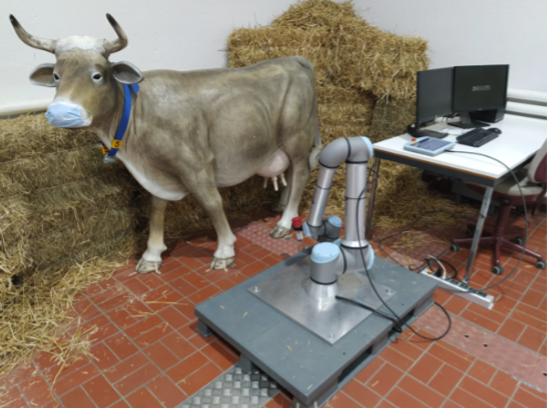
\includegraphics[width=0.7\textwidth]{images/cow_setup.png}
        \caption{Artificial cow setup at the ZHAW}
        \label{fig:cow_setup}
    \end{figure}
    
    \begin{itemize}
        \item \textbf{Blackbox PC:} where the Robot Operating System was running the pose estimation and the robot manipulation.
        \item \textbf{UR10e robot:} industrial robot used in machine tending, palletizing, and packaging (6 axis).
        \item \textbf{Arm Flange:} the flange at the end of the arm had the camera and the milking cup.
        \item \textbf{Dummy cow:} artificial cow model with fake teats to test the robotic attachment.
    \end{itemize}
   
    
    An important aspect in the physical setup for the given task is the specific camera characteristics. A camera can have different performances as a factor to light conditions, shifting, object colors, glass panels and lower resolutions. Given the systemic error a camera can introduce, it is essential to minimize the influence of it. Therefore, a camera evaluation was carried out to compare diverse camera manufacturers and models. Appendix \ref{appendix:camera_evaluation} illustrates the performance of different cameras that were available for evaluation, and presents a clear model that outperforms the rest. 

\newpage
\section{Pipeline Deployment}\label{chap:4:deployment}
The deployment of the components was done using docker compose files to leverage the capabilities of microservices, where every component used behaves as a separate component in the application. The benefit gotten out of microservices is that they are small in size, bounded by their context, independently developed and deployable and they allow for message-based communication%todo ADD REF
. 
% For the deployment of the pipeline on the GPU servers, docker images were built per component (RViz, ROSPlay, ROSTeat, PoseEstimator, etc.). A set of docker compose files was used to control the deployment of the docker containers. 
Figure \ref{fig:cow_docker_topology} shows a sample docker-compose file, which describes the services and the volumes being deployed. In this particular example, Pose Estimator waits for ROSTeat to be succesfully deployed, whereas ROSTeat waits for ROSPlay.

\begin{figure}[h]
    \centering
    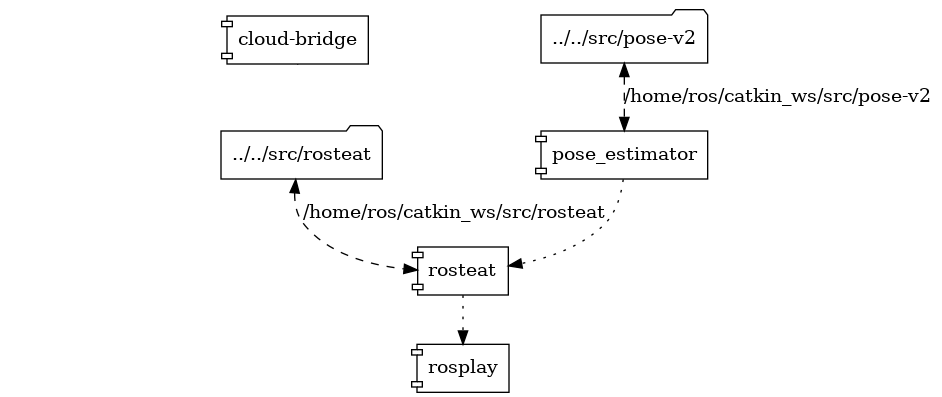
\includegraphics[width=1\textwidth]{images/cow_docker_topology.png}
    \caption{Example of a Docker-compose Deployment}
    \label{fig:cow_docker_topology}
\end{figure}

The components proposed in the previous Chapter were developed both in Python 2.7 and 3.6, which was not an obstacle given the modular approach. The only problem encountered were the outdated packages given that Python 2.7 has been deprecated as of January 1st, 2020. 
Aditionally, the set of libraries and tools used for developing the pose estimation component in the Robot Base was the Robot Operating System (ROS). "ROS provides the services you would expect from an operating system, including hardware abstraction, low-level device control, implementation of commonly-used functionality, message-passing between processes, and package management" \cite{2020ROS}. In this sense, the specific version of ROS used for the development were ROS Melodic and ROS Noetic.


\section{Segmentation Network Training}\label{chap:4:train_data}

The training data was collected using the robot's base recording procedure, which stores the set of input frames observed as a video file in ROS format (ROSbag), which could be replayed for future testing or simulations. Rviz can then be used to collect the RGB images and depth images at manually indicated timestamps. The RGB-D input received from the camera consists of images with a resolution of 640 x 480 x 4 pixels. 
% Each pose estimation algorithm receives the input from the camera and the segmentation mask and processes it differently. 
% This was done to analyze the precision from different sources of information (for example, point cloud versus depth image).

\begin{figure}[h]
    \centering
    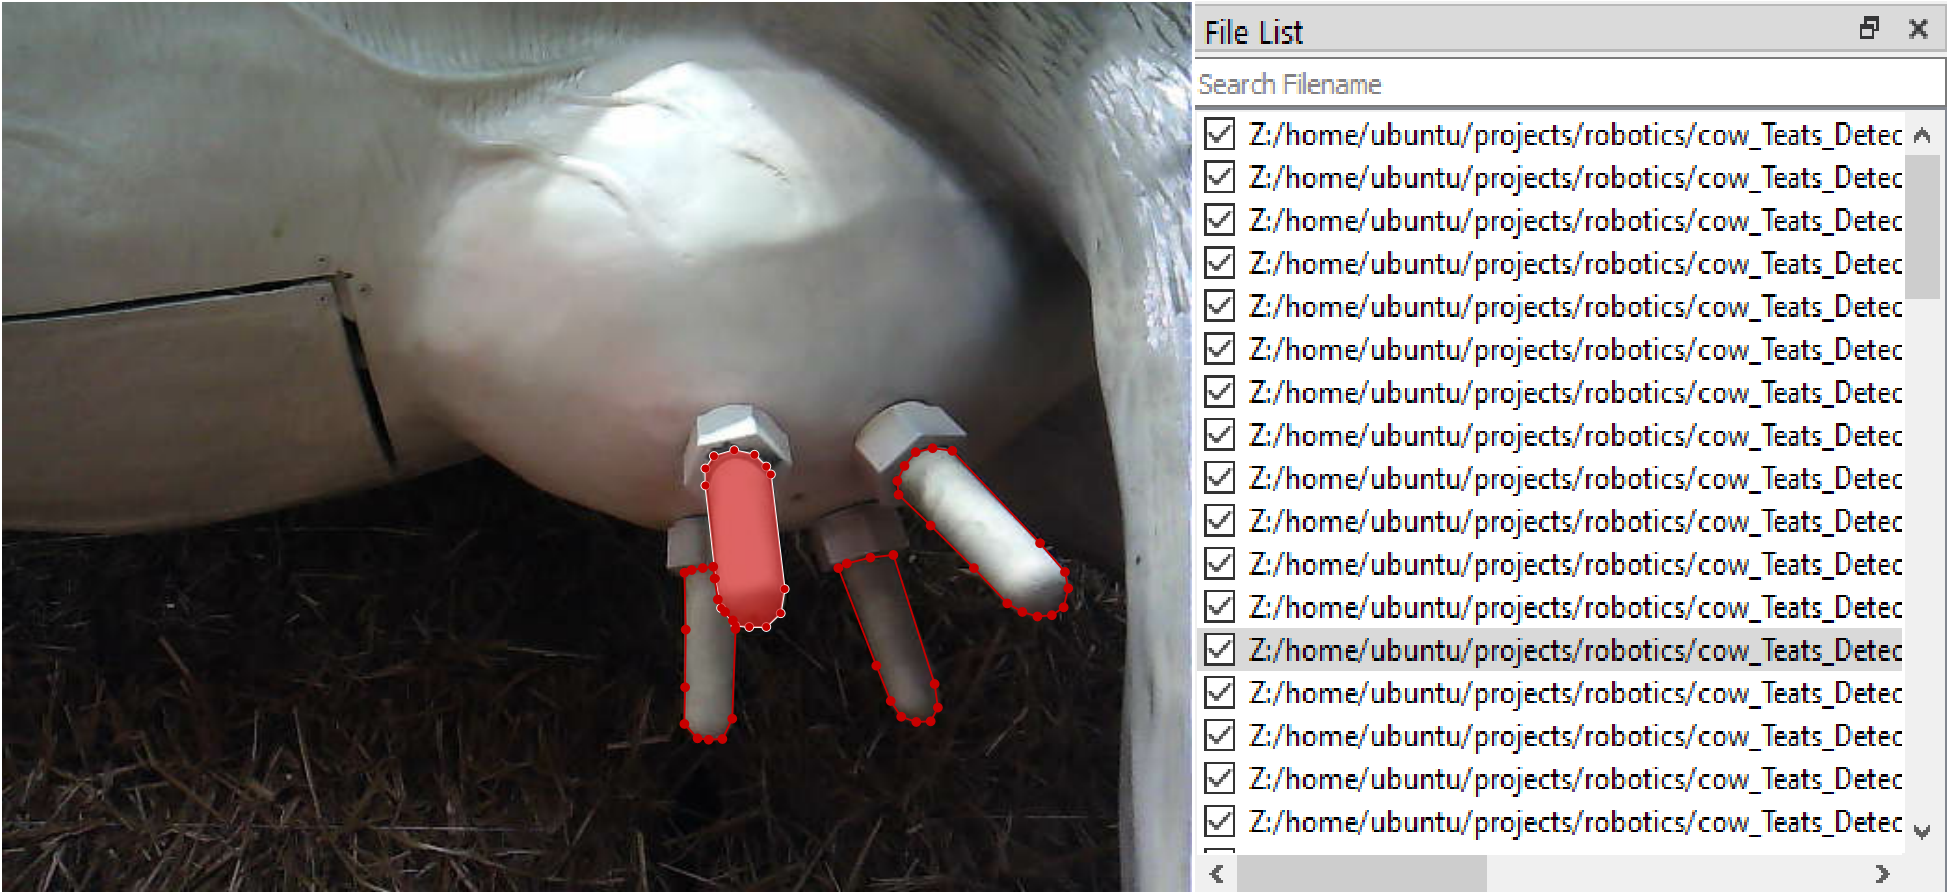
\includegraphics[width=0.4\textwidth]{images/cow_labelme.png}
    \caption{Image annotation example.}
    \label{fig:cow_labelme}
\end{figure}
The collected realistic images are then imported into the image annotation tool LabelMe\cite{2021labelme}. Labelme is used to manually mark the pixel-wise segmentation areas and to assign the class labels.  Figure \ref{fig:cow_labelme} shows a glimpse of the labelling tool. Once an image has been labelled the pixel-wise segmentation is stored as a polygon in JSON file next to the original image. As a final step, a Python script is used to merge all the individual JSON files into one, before feeding the data set into the network for training.

\begin{longtable}{@{} p{8cm} c @{}} \toprule
% \textbf{asd}       & \textbf{Segment Cow Teats from Image} \\ \midrule
Number of Synthetic Training Images generated                   & 400'000 \\ \cmidrule{1-2}
Number of Synthetic Validation Images generated                   & 20'000 \\ \cmidrule{1-2}
Number of Realistic Training Photos collected             & 192 \\ \cmidrule{1-2}
Number of Realistic Validation Photos collected             & 192 \\ \cmidrule{1-2}
Total Number of Features                    & 1 \\ \bottomrule
\caption{Data sets statistics.} \label{tab:dataset-statistics} \\
\end{longtable}

The network training was performed on an NVIDIA Tesla T4 GPU\cite{2021testat4}.
% with 16 GB VRAM. 
CUDA\cite{2021nvidia-cuda} was used to parallelize the computations both in training and testing, and therefore speed up the processing times. Table \ref{tab:dataset-statistics} provides an overview of the data set statistics used for training. 
Additionally, the docker images were configured so that the training parameters can be input as environment variables. These parameters include the data set, local weights and the remote weights locations, the epochs, score threshold, learning rate, etc. Table \ref{tab:train-results} show the classification errors of the methods trained

\begin{longtable}{@{} p{5cm} C{2cm}           C{2.5cm}                   C{1.5cm}           C{1.5cm}         @{}} \toprule
\textbf{Method}              & \textbf{Dataset} & \textbf{Learning rate}   & \textbf{Epochs}  & \textbf{Accuracy}  \\ \midrule
matterport/MaskRCNN - Py2.7         & Realistic        & 0.002                    &  100             & 97\%          \\ \midrule
matterport/MaskRCNN - Py3.6         & Realistic        & 0.002                    &  100             & 97\%          \\ \midrule
Detectron2/MaskRCNN                 & Realistic        & 0.00025                  &  2000            & 98\%          \\ \midrule
Detectron2/MaskRCNN                 & Synthetic        & 0.00025                  &  2000            & 0\%          \\ \bottomrule
\caption{Segmentation networks performance.} \label{tab:train-results}
\end{longtable}


As shown above, the synthetic data set proved the images were not photorealistic enough to close the reality gap. Both the matterport and the Detectron2 implementations of MaskRCNN showed similar accuracy. However, the implementation from matterport in Python 2.7 had an initial average loading time of 40 seconds and the implementation in Python 3.6 had a 4 seconds average loading time. Moreover, benchmarks show the implementations from matterport have a 4x slower throughput (imgs/sec) compared to Detectron2 \cite{2021detectron2-benchmark}. These drawbacks and the generally better performance of the Detectron2 implementation led to it being chosen for the segmentation task. 
% Finally, the increase of the prediction score threshold was the only optimization done, other than the parameters shown in Table \ref{tab:train-results}.

\section{Results} \label{chap:4:results}
\subsection{Research Question}
\label{sec:results-research-question}
% \lipsum[1-4]

The research question tackles the pose estimation of cow teats. This section will describe the results obtained for each approach proposed, along with their respective optimizations. 

Table \ref{tab:test-results} provides a brief summary of the results and the general performance of the used algorithms, which are discussed afterwards in more detail.

\begin{longtable}
{@{} l c c @{}} \toprule
\textbf{Method}                     & \textbf{Accuracy}     & \textbf{Standard Deviation}       \\ \midrule
% PCA                                 & 97\%                  & 0.015                             \\ \midrule
MAV                                 & \textbf{97\% }                 & \textbf{0.43}                             \\ \midrule
DOPE                                & 0\%                  & -                             \\ \midrule
RANSAC                              & 0\%                   & -                             \\ \bottomrule
\caption{Statistics of tested methods.} \label{tab:test-results}                          \\
\end{longtable}

% The following Table displays the results for the PCA-variant algorithm. The variants presented are optimized by modifying the offset and the averaging mechanism used to calculate the Teat Tip coordinates.
% \begin{longtable}{|p{1.5cm}|p{3cm}|C{1.5cm}|}                                              \hline
% \multicolumn{3}{|l|}{\textbf{PCA-variant}}                                                       \\\hline
% \textbf{Offset}         & \textbf{Averaging Method}   & \textbf{Accuracy}                \\ \hline
% Fixed                   & Single Point                & 97\%                             \\ \hline
% Mixed                   & Single Point                & 97\%                             \\ \hline
% Fixed                   & Average: 1/3rd              & 97\%                             \\ \hline
% Mixed                   & Average: 1/10th             & 97\%                             \\ \hline
% \caption{Overview of the best MAV results for the respective offset-averaging mechanisms combinations.} \label{tab:test-results}                          
% \end{longtable}

% The following Table displays the results for the Normals algorithm. The variants presented are optimized by modifying the offset and the averaging mechanism used to calculate the Teat Tip coordinates.
% \begin{longtable}{|p{1.5cm}|p{3cm}|C{1.5cm}|}                                              \hline
% \multicolumn{3}{|l|}{\textbf{Normals}}                                                       \\\hline
% \textbf{Offset}         & \textbf{Averaging Method}   & \textbf{Accuracy}                \\ \hline
% Fixed                   & Single Point                & 97\%                             \\ \hline
% Mixed                   & Single Point                & 97\%                             \\ \hline
% Fixed                   & Average: 1/3rd              & 97\%                             \\ \hline
% Mixed                   & Average: 1/10th             & 97\%                             \\ \hline
% \caption{Overview of the best MAV results for the respective offset-averaging mechanisms combinations.} \label{tab:test-results}                          
% \end{longtable}

The following Table \ref{tab:DOPE-results} displays the results for the DOPE algorithm. DOPE uses FAT formatted data sets, which are generated using NDDS, in Unreal Engine 4. These data sets are characterized for being synthetic photorealistic images. The data set variants presented below are optimized by modifying the parameters in data set used, such as:
% The variants used include changes in: 
the realism degree in the materials used for the object textures, the usage of rotation in the focus object, and the usage of obstructive objects. Aditionally, all data sets include five different photorealistic scenes: beach, studio, temple, meadow and zen garden. Surprisingly none of the data sets were realistic enough to close the reality gap, which reflected in DOPE not outputting any predictions.

\begin{longtable}{|l|c||c|}                            \hline
\multicolumn{3}{|l|}{\textbf{Deep Object Pose}}              \\\hline
\textbf{Dataset}            & \textbf{Size}  & \textbf{Functional}            \\ \hline
NDDS Realistic (base)       & 260k      & No                             \\ \hline
NDDS Realistic 2.0          & 80k       & No                             \\ \hline
NDDS with Obstruction       & 80k       & No                             \\ \hline
NDDS with Rotation          & 80k       & No                             \\ \hline
NDDS Small                  & 20k       & No                             \\ \hline
\caption{Overview of the best DOPE results for the respective dataset variations.} \label{tab:DOPE-results}
\end{longtable}

The results for the RANSAC algorithm are shown in Table \ref{tab:ransac-results}. The skimage implementation was used for both RANSAC and direct ORB matching. The variants presented were surprinsingly not succesful at matching the cow teats patterns. It is suspected that RANSAC and ORB matching are not the best approach for identifying simple texture objects such as the cow teats. 
Figure \ref{fig:ransac-results} illustrates the suspicion and the behavior of RANSAC on both the RGB and the depth images. RANSAC was tested by varying the ORB number of keypoints, the ORB threshold and RANSAC's residual threshold as well as adding a denoising step.  
% \begin{longtable}{|p{1.5cm}|p{3cm}|C{1.5cm}|}                                              \hline
% \multicolumn{3}{|l|}{\textbf{RANSAC}}                                                       \\\hline
% \textbf{Offset}         & \textbf{Averaging Method}   & \textbf{Functional}                \\ \hline
% Fixed                   & Single Point                & No\%                             \\ \hline
% Mixed                   & Single Point                & No\%                             \\ \hline
% Fixed                   & Average: 1/3rd              & No\%                             \\ \hline
% Mixed                   & Average: 1/10th             & No\%                             \\ \hline
% \caption{Overview of the best MAV results for the respective offset-averaging mechanisms combinations.} \label{tab:test-results}                          
% \end{longtable}
\begin{longtable}{|c|c|c|c||c|}                            \hline
\multicolumn{5}{|l|}{\textbf{RANSAC / ORB Matching}}              \\\hline
\textbf{ORB \#keypoints} & \textbf{ORB threshold} & \textbf{Residual Threshold} & \textbf{Denoising}       & \textbf{Functional}      \\ \hline
        20      & 0.08      & N/A (ORB matching)       & No     &  No               \\ \hline
        200     & 0.08      & N/A (ORB matching)       & No     &  No               \\ \hline
        200     & 0.02      & 0.5       & No     &  No               \\ \hline
        200     & 0.02      & 0.5       & Yes    &  No               \\ \hline
        200     & 0.02      & 0.9       & No     &  No               \\ \hline
        200     & 0.02      & 0.9       & Yes    &  No               \\ \hline
        200     & 0.08      & 0.5       & No     &  No               \\ \hline
        200     & 0.08      & 0.5       & Yes    &  No               \\ \hline
        200     & 0.08      & 0.9       & No     &  No               \\ \hline
        200     & 0.08      & 0.9       & Yes    &  No               \\ \hline
\caption{Overview of the best MAV results for the respective offset-averaging mechanisms combinations.} \label{tab:ransac-results}                          
\end{longtable}

 \begin{figure}[h]
        \centering
        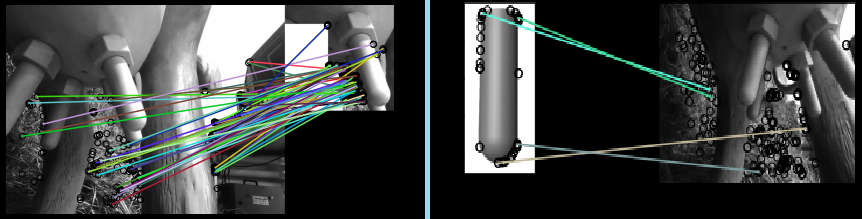
\includegraphics[width=0.9\textwidth]{images/cow_ransac.png}
        \caption{RANSAC's behavior on the cow data set.}
        \label{fig:ransac-results}
    \end{figure}
    
The following table 
% \ref{tab:mav-results} displays 
presents the results for the "MAV" algorithm. The algorithm leverages the segmentation mask and overlays it over the depth image. Afterwards, the 2D points are proyected into 3D space and PCA is used to calculate the teat direction. Finally, the N points (averaging method) at the bottom of the teat (using the direction indicated by PCA's first component) are averaged to obtain a "teat's tip coordinates". A manual offset was added to the obtained coordinates to attempt to fix the (x,y,z) error observed. The MAV optimizations presented are a combination of the offset and the averaging method.

\begin{longtable}{|l|l||c|c|c|}                                              \hline
\multicolumn{5}{|l|}{\textbf{MAV}}                                                       \\\hline
\textbf{Offset}         & \textbf{Averaging Method}   
& \textbf{Average Error}  & \textbf{Standard Deviation}  & \textbf{Execution Time}                 \\ \hline
Fixed                   & Single Point                & 1.13            & 2.8              & 0.26 - 1.5 secs   \\ \hline
Calculated              & Single Point                & 1.77            & 3.3              & 0.26 - 1.5 secs   \\ \hline
Fixed                   & Average: 1/3rd              & \textbf{0.67}   & \textbf{2.4}     & 0.26 - 1.5 secs                     \\ \hline
Calculated              & Average: 1/3rd              & 1.54            & 2.93             & 0.26 - 1.5 secs    \\ \hline
Fixed                   & Average: 1/10th             & 0.96            & 2.55             & 0.26 - 1.5 secs     \\ \hline
Calculated              & Average: 1/10th             & 1.51            & 2.87             & 0.26 - 1.5 secs    \\ \hline
\caption{Overview of the best MAV results for the respective offset-averaging mechanisms combinations.} \label{tab:mav-results}                          
\end{longtable}

% \subsection{Research Question 2}

% The second research question tackles the evaluation of the pose estimation of cow teats.

% \subsection{Quality Ranking of Predictions}
\subsection{Deliverables}
The following deliverables will be handled in with this Vertiefungsarbeit:
\begin{itemize}
    \item This work produced a pose estimation system, which is able to estimate a cow teat's pose with an average error of 0.67 cm and a standard deviation of 2.4 cm. 
    \item This work also contributed to two other variations of the MAV algorithm that were developed by the project team for the cow teats project.
    \item For future research, an Unreal Engine 4 project with 5 different photorealistic scenes for a synthetic data set generation, including a cow teats data set containing over 400k images for pose estimation.
\end{itemize}
\chapter{Discussion}\label{chap:discussion}
This chapter will discuss the obtained results, the used methodology, the validity and the reliability of the experiments, adapting the structure proposed by \textcite{luckert2016using}. Section \ref{sec:results-interpretation} will look into the results, describing what has been achieved, as well as indicate the main problems concerning the experiments. Section \ref{sec:method-reflection} will reflect on the research task and discuss whether the right method was chosen to solve the given task. Finally, Section \ref{sec:results-reliability} discusses the validity of the datasets that were used and the overall experiment setup. Based on these validity remarks, this chapter will clarify the reliability of the experiments' results. Therefore, the following questions will be tackled:
\begin{itemize}
    \item What conclusions can be taken from the presented results?
    \item Was the chosen method appropriate for the task?
    \item What benefits and shortcomings have been identified related to the presented work?
    \item What is the validity and reliability of the used data sets and the presented results?
\end{itemize}

\section{Results Interpretation}\label{sec:results-interpretation}
The best results among all algorithms were achieved by the manual manipulation of features "MAV", with a 0.67 cm error with a standard deviation of 2.46. The variations of MAV do not show substantial differences, yet they all present an average error higher than 0.5 mm with respect to the ground truth. 

This contrasts with the performance shown by the other two algorithms: RANSAC and DOPE. First, RANSAC could not match the pixel descriptors for the cow teats in the RGB images as shown in Section \ref{sec:results-research-question}. It is suspected that RANSAC could show better results if some preprocessing is done on the depth images. In other words, if the hypothesis that RANSAC cannot match figures of uniform colors from the RGB image, then a better performance could be seen when processing the depth image or the point cloud, as other research proposes \cite{papazov2010efficient}. Second, DOPE's performance was unexpected since it was used before for 3D recognition of chairs at the ZHAW and it showed promising results. It is suspected that DOPE's disappointing performance is originated because of the lack of photorealism in the materials of the data sets. Since the artificial cow teats materials are not a plain "gray", it was difficult to close the reality gap with simple materials. The hypothesis for improvement is that DOPE should show a better performance if the reality gap in the data set is minimized further.


An additional point of improvement would be a mechanism to reduce the offset error shown by "MAV". The correlogram shown in Appendix \ref{appendix:correlogram} was generated with the outputs from the algorithm, to obtain the correlation coefficients between the errors in (x, y, z) with the camera position (x, y, z) and the camera's direction (quaternion). The coefficients proved there is a strong indirect correlation between the errors and the camera metrics. Consequently, a linear model was fit to predict the errors based on the interaction of camera information variables. The model's adjusted R-squared shows that 94\% of the variation in the output variables is explained by the input variables. Additionally, the overall F-statistic of the model show that the model indeed provides a better fit than the intercept-only model. Finally, as shown in Figure \ref{fig:r_error_asf_xyzquat}, the model's residuals were analyzed. These show a constant error, constant variance, normal distribution and no influential outliers. All these cues hint towards the possibility of using a linear model to predict the error in the "MAV" algorithm to reduce the offset error in the final pose estimations.

 \begin{figure}[h]
        \centering
        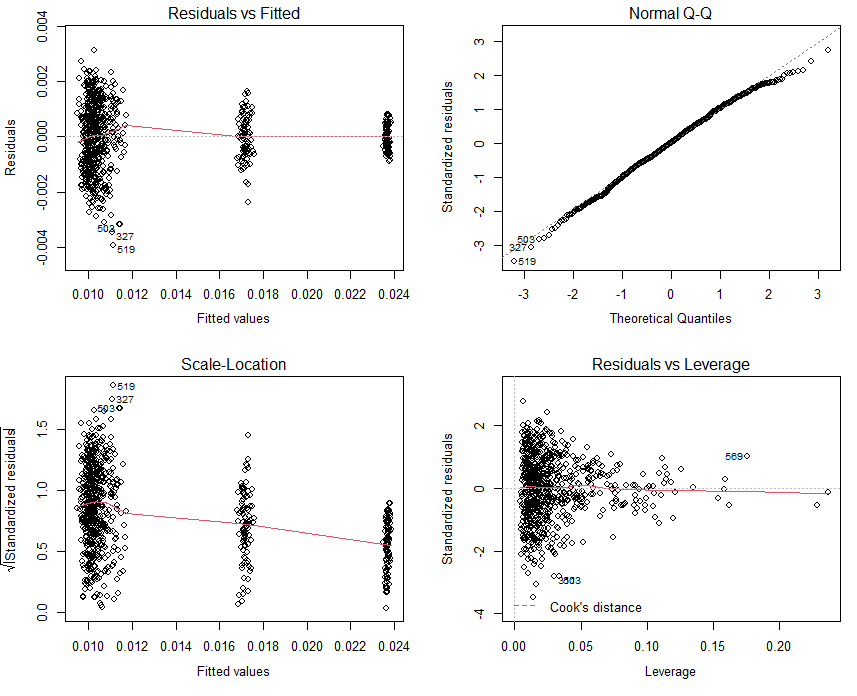
\includegraphics[width=0.8\textwidth]{images/r_error_asf_xyzquat.png}
        \caption{Linear model residuals of the model fit to predict the error from "MAV".}
        \label{fig:r_error_asf_xyzquat}
\end{figure}
    


\section{Method Reflection}\label{sec:method-reflection}
The used method, adapted from the work by \cite{luckert2016using}, proved to be appropriate for proposing a solution for the research question given. The structure provided allowed for the setup of different experiments without neglecting the initial goal. From the identification of the goal, through the data description and the specification and proposition of the computer vision approaches, the method proved to efficiently structure the work required to construct a pose estimation algorithm using machine learning.

\section{Reliability}\label{sec:results-reliability}
This section aims to discuss the validity and reliability of the results shown in section \ref{sec:results-research-question}.

The achieved results by the pose estimation algorithm, specially the adaptations done in contribution based off this work, show better performance than the methods in the market for the cow milking robots. The obtained results show promising a performance for current challenges like detecting two cow teats as one. Once the error in the proposed method is reduced, the proposed pipeline could be connected to a memory system that would keep track of the cow teat positions in cases of obstruction from the suction cups, as discussed in Section \ref{sec:future-work}.

In contrast, a few shortcomings related to the achieved results must be mentioned. First, the RANSAC algorithm analysis was limited to RGB images and should have been expanded to evaluate the information from the depth image and the point cloud. Second, a more photorealistic data set should be generated to show DOPE's prediction capabilities and carry out a proper comparison with the "MAV" algorithm. Third, the search space of the parameters adjusted should be wider and not limited to the ones presented. In conclusion, the "MAV" algorithm answers the research question with success, being able estimate the 3D pose and direction of a cow teat in less than 2 seconds.

\chapter{Conclusion}\label{chap:conclusion}
\section{Conclusions}\label{sec:conclusions}
This work answered the following research question:
\begin{itemize}
    \item How can the cow teats 3D pose be estimated under 10 seconds?
\end{itemize}
This was done by constructing a data set, training a segmentation algorithm and estimating the pose of the cow teats from the image and the predicted segementation masks. The images for the data set were collected from an artificial cow at the ZHAW using ROSBags to manually export frames at specific timestamps. The images were subsequently annotated and added to the data set. The model was then trained and tested using the generated data set. The false negatives and false positives indicated that more pictures at specific time stamps and positions with respect to the artificial cow had to be added to the data set, to increase the model's accuracy. Consequently, a pipeline was constructed for the independent deployment of the segmentation network and the pose estimation algorithms. The segmentation network would predict and publish segmentation masks for the pose estimation component to consume them and predict, in conjunction with the input images, the pose estimation of the observed cow teats. The methods tested were RANSAC and a manual manipulation approach "MAV". The latter contributed to two other approaches at the ZHAW for the pose estimation of cow teats. From the methods presented in this work, the best results were by a manual approach "MAV", which had a 0.67 cm error with a standard deviation of 2.46. 

Additionally, an Unreal Engine 4 project for data set generation was constructed for further research. It contains 5 photorealistic scenes with present parameters for rotations and obstructing objects. Finally, a synthetic data set of cow teats was generated with over 400k images for pose estimation. This dataset was used to train the pose estimation algoritmh DOPE, which unfortunately could not close the reality gap and output predictions from real images.

\section{Where to Go From Here?}\label{sec:future-work}
This work presents a pose estimation system for cow teats using machine learning and computer vision methods. There are a few possible routes for the extension of this work to improve the performance of the achieved results. First, a different segmentation network with a faster prediction time could significantly reduce the overall performance time of the presented approach, leading to almost real-time performance. Second, a memory system could help in cases of obstruction. For example, when the suction cups are attached, the system could still remember the position of the cow teats and attempt to reattach in case one of the cups detached on movement. Third, an active vision system could significantly improve the algorithm's time to obtain precise predictions. An active vision system would control the camera position and movement to collect frames with the least amount of movements, so that the objects in the scene could be remembered and understood more efficiently.

In conclusion, the presented work extends the related research on this topic by a providing machine learning and computer vision based approach for the 3D pose and direction estimation of cow teats.

% In this work we could show that is it possible to acquire a deep scene understanding from sequential
% data with supervised learning. In a simplified use-case such as the presented one, the system can
% successfully acquire a spatial scene understanding that includes objects, their shape, color and even
% their relationship with other objects. Although it is limited to the type of scenes the system was trained
% on, its versatility exceeds by far current mainstream object recognition systems such as ResNet [6].
% Unlike encoder-decoder-based scene understanding approaches such as [32], we do not need specified
% 3D models for training but only a simple scene description that specifies present objects including their
% positions and the camera poses of the captured images. 

% We could show that our system is capable of
% sequentially integrating information from new frames into the existing scene embedding vector. This
% capability is indeed highly remarkable because it includes the achievement of multiple non-trivial steps:
% 1.The change in camera position relative to the previous frame needs to be evaluated. The system does
% not receive any information about the camera position or rotation in space, but needs to extract this
% information based on the difference between the already perceived and the new input frame.2.This
% extracted transformation of the camera position must be used to transform all remembered object
% positions. Some objects might be occluded by the obstacle or other present objects, and the system is
% not able to perceive these items in the current frame. Nonetheless, it is necessary to transform their
% remembered positions so that the system is able to return the correct position when queried. The
% precision of this process however, would need to be further improved when used for robotic grasping,
% as there is still an average deviation of 0.11 meters (about half the diameter of the object) from the
% ground truth when using the best performing approach.

% While our proposed system does not use separated streams for ventral and dorsal pathways, our information
% aggregation process is inspired by the quicker decaying dorsal memory and the more persistent
% ventral memory. This is represented by learned weights versus aggregated temporary information. This
% architecture seems to work great, especially with respect to the 3 different shortcomings that were the
% focus of this work (see section 1.2). In the following, we discuss how our system overcomes them:
%     % \begin{itemize}
%     %     \item 1 paragraph big: describe what was achieved
%     %     \item 1 paragraph: describe our limitations
%     %     \item describe how we "overcame" the shortcommings: 3 paragraphs
%     %     \item closing remarks
%     % \end{itemize}


% \section{Towards Active Vision}
% Since this work was initially inspired by robotic interaction, we would see it as the next step to combine
% our vision-focused system with grasping approaches. An interesting direction would be to work towards
% solving benchmarks for robotic interaction such as RLBench [59].

% When approaching such tasks, we mainly see two possible paths to take: One relatively simple way
% would be to keep the perception and the grasping system separate and only use the output of the
% presented approach as input for a grasp generation algorithm, such as Dex-Net [60]. This would mean
% that the perception part would identify the target object and then forward its position to the grasp
% planning mechanism which would plan the grasp and pass it to the robotic arm for execution. As
% second option it would be possible that the condensed scene representation produced by our system
% would be beneficial for grasp-generation. We think that a promising approach would be to train two
% streams for grasping. The first stream could create a large number of possible grasps, while the other
% one would rate them with likelihood of success. Of course, the system would first need to learn to
% include the required information in the scene representation, which might be a large leap compared to
% the information currently present within the trained system. However, with the human mind closely
% coupling perception and action as part of the dorsal pathway it seems that such a joint approach could
% work for robotic grasping too.
%     % \begin{itemize}
%     %     \item 1 big paragraph describing how active vision could improve accuracy and object permanence
%     % \end{itemize}
% \section{Where to Go From Here?}
% While the discussed approach successfully solves the tasks set, the system is still far from being a real
% replacement for existing computer vision algorithms in use. On the way to the application of a system
% like ours to solve tasks in the real world, it would be necessary to solve at least some of the following
% challenges:

% Real world data: In order to use an approach like the one presented in a real-world use-case, it would
% above all be necessary to transfer the approach to real data or at least more realistic synthetic data.
% With the goal to jointly improve both scene understanding and active vision, we would inspire future
% research to use real-time data gathering with simulated environments as for example Isaac Sim [61].
% This would allow non-discrete view-positions and thus a potentially better understanding. One aspect
% that still might not be solvable by using synthetic data is the noise of the depth-channel of the RGB-D
% data, which is quite prominent for most consumer class RGB-D-camera.

% More different object classes/shapes: The presented solution uses only 5 primitive shapes with 7
% colors, which most likely does not reflect the conditions of a real world use case. A possible solution
% could be the use of large-scale 3D object data sets as used for Dex-Net [60]. Closely related to more
% diverse objects would be the capability to deal with duplicate objects. This could possibly be solved by
% adding multi-object output to all streams (as demonstrated with the Enumerating stream).

% Motion: In this work, we did not address the topic of motion, which does play a big roll in the real
% world. Environments like conveyor belts would be a domain where a scene understanding system like
% the one presented could prove highly useful. However, an application in such an environment would
% require previous research with dynamic scenes.

% Rotation axis detection: With only primitive objects such as cube, cylinders, etc., we decided not to
% include rotation information for our streams. However, for a large number of use cases it could be very
% useful to obtain the rotation of an object, so we would encourage future work to extend our approach
% to include rotation information.
% Grasping/bounding-box detection: For an actual application of robotic grasping, it would be necessary
% to generate possible grasping positions. We did not address this topic in the course of this work
% but leave the extension of the presented approach with grasping to further research. For more details
% see section 5.3.
%     % \begin{itemize}
%     %     \item describe in 5 small paragraphs 5 different future improvements for the voerall system
%     % \end{itemize}




%% Use letters for the chapter numbers of the appendices.
\appendix

\begin{RaggedRight}
	\bibliography{report.bib}
\end{RaggedRight}
\newpage

\listoffigures
\listoftables

\chapter{Appendix}\label{sec:chapAppendix}
\setheader{Appendix}

\section{Contact Information and Code Access}
If you have any questions regarding this work, feel free to contact me at j.francisco.ribera@gmail.com. Given that the Melkroboter proyect is looking to request Patent rights, the code might not be available for public access.
% \section{Other Algorithm Evaluations}
%     \begin{itemize}
%         \item DOPE performance
%     \end{itemize}
% \section{Official Assignment}
% TODO: copy paste from moodle

\newpage
\section{Synthetic Dataset Generation Overview}
\label{appendix:ndds}

\begin{figure}[!ht]
    \centering
    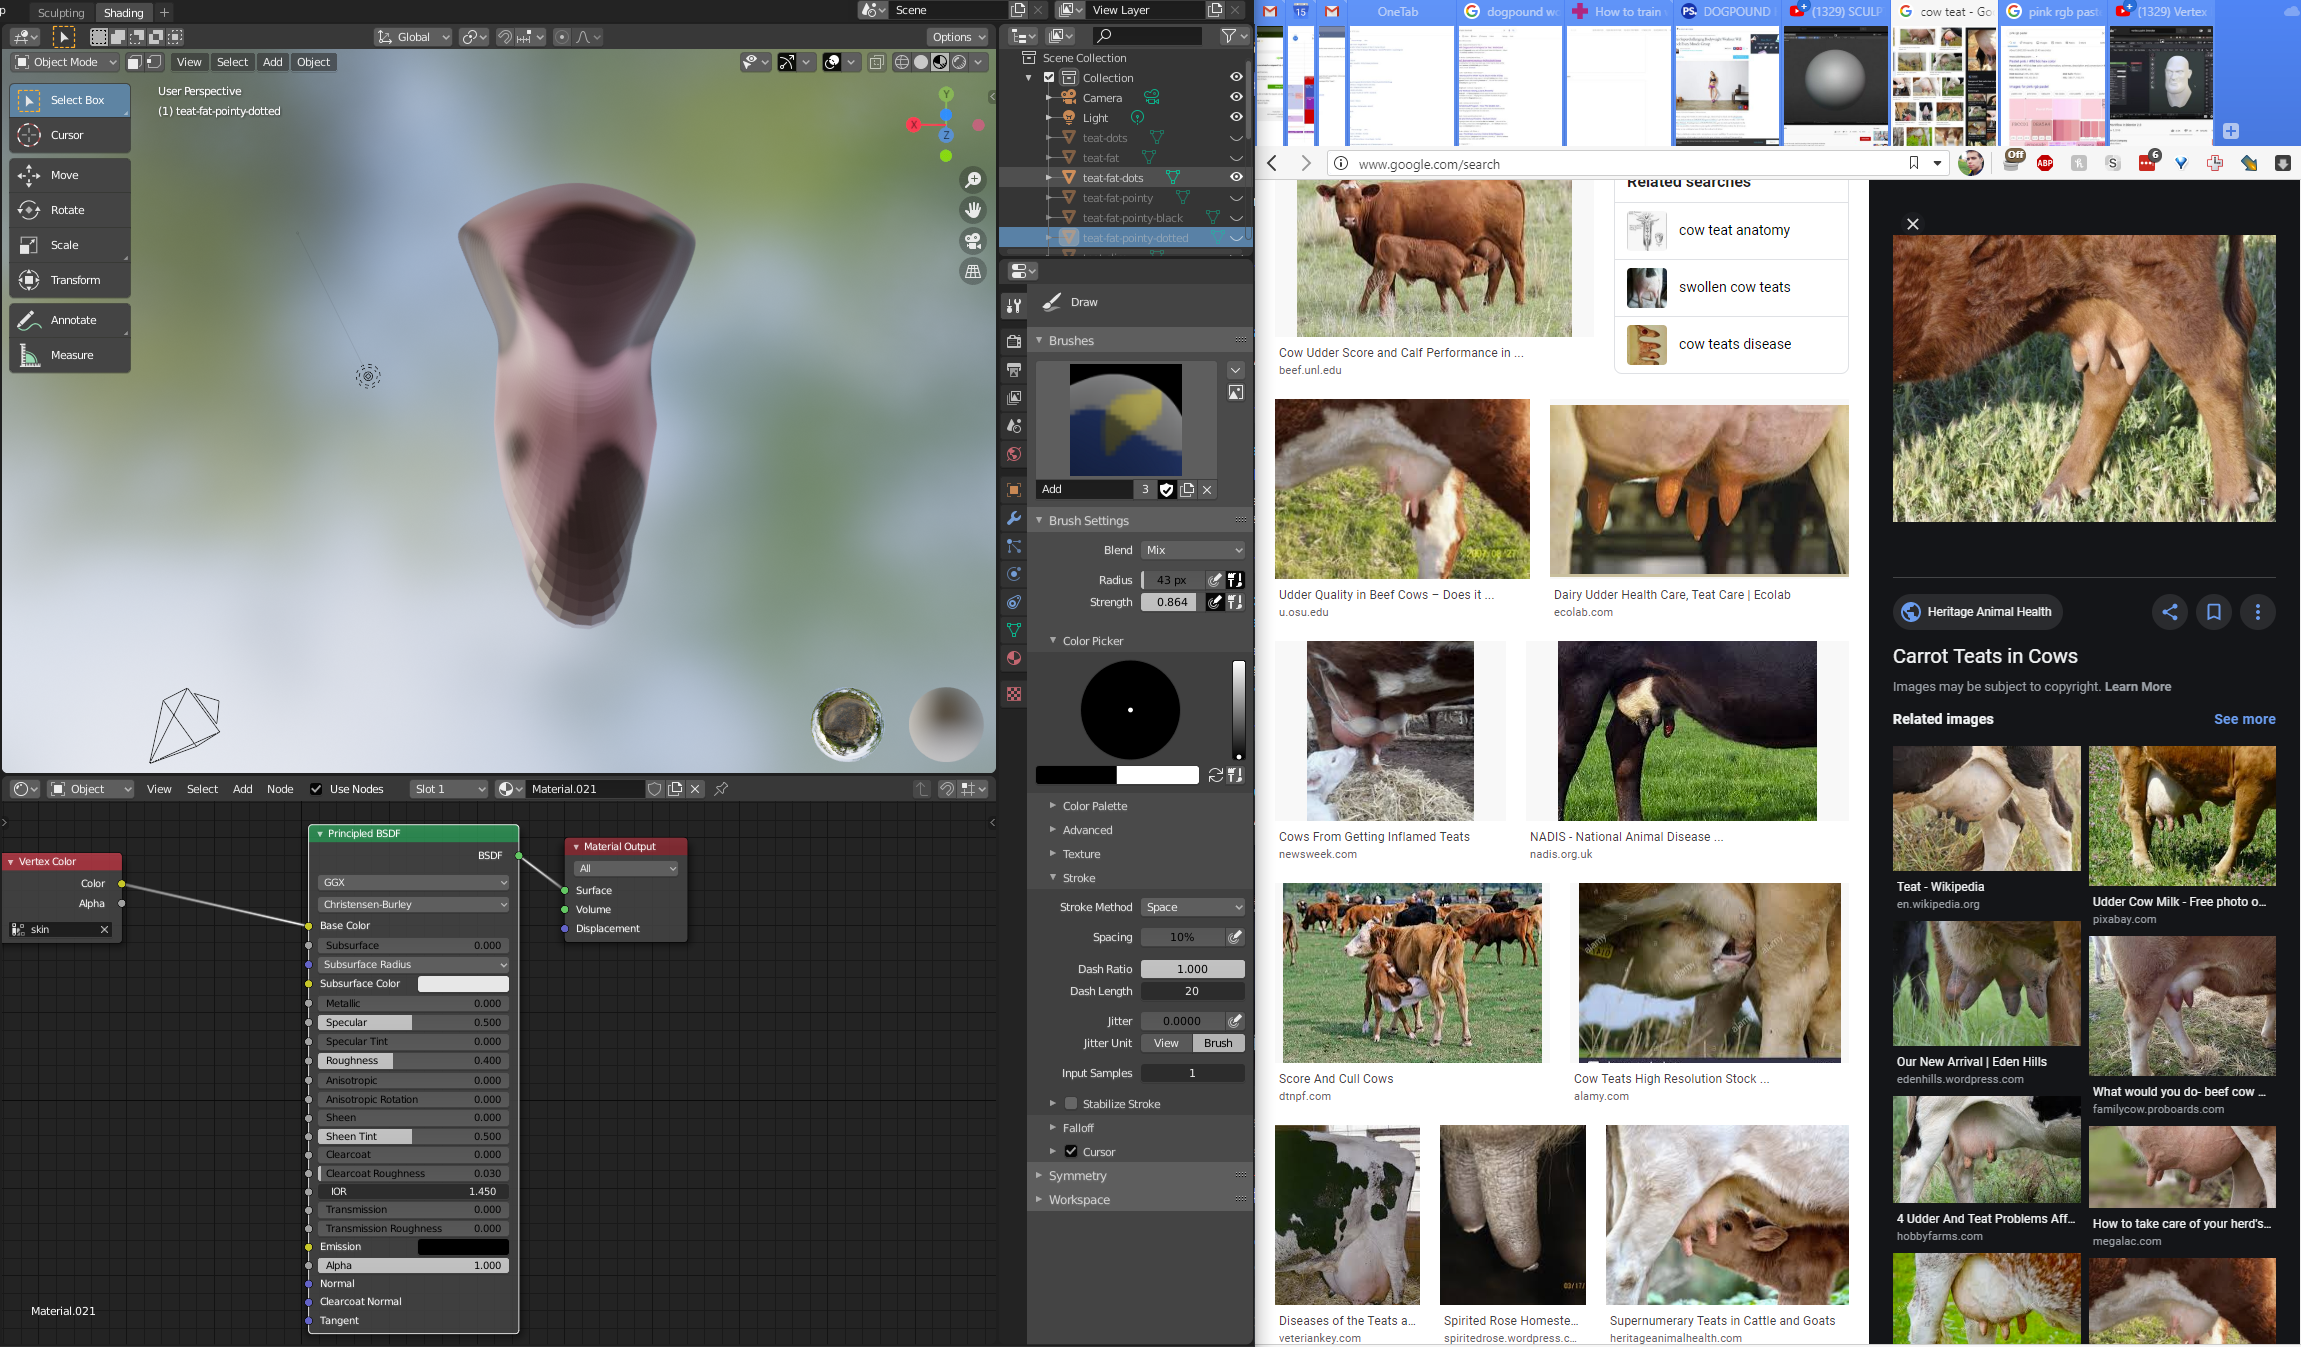
\includegraphics[width=.8\textwidth]{images/ndds1}
    \caption{Screenshot of a photorealistic scene in Unreal Engine 4.}
    \label{fig:ue4-1}
\end{figure}
\begin{figure}[!ht]
    \centering
    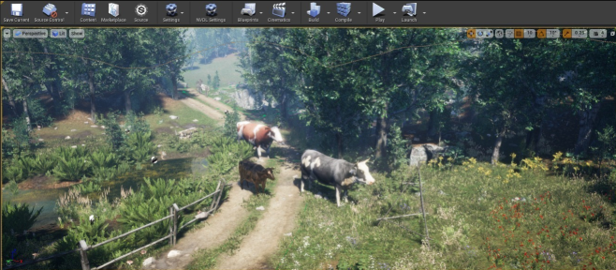
\includegraphics[width=.8\textwidth]{images/ndds2}
    \caption{Screenshot of a photorealistic scene in Unreal Engine 4.}
    \label{fig:ue4-2}
\end{figure}
\begin{figure}[!ht]
    \centering
    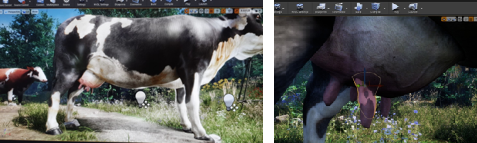
\includegraphics[width=0.8\textwidth]{images/ndds3}
    \caption{Screenshot of a photorealistic scene in Unreal Engine 4.}
    \label{fig:ue4-3}
\end{figure}
% \begin{figure}[!ht]
%     \centering
%     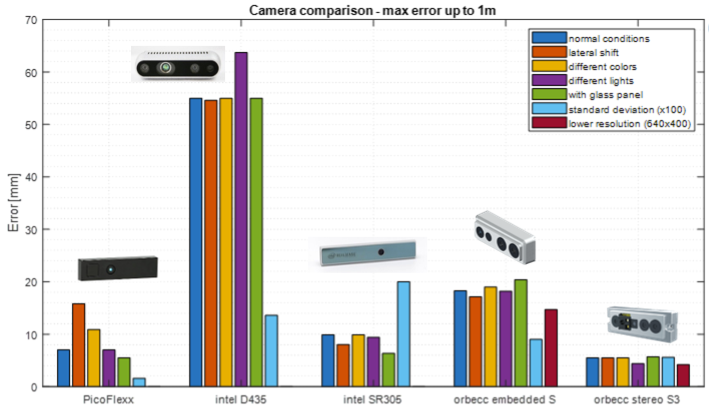
\includegraphics[width=1\textwidth]{images/camera_choice.png}
%     \caption{Screenshot of a sample export from the NDDS plugin.}
%     \label{fig:ndds}
% \end{figure}

\newpage
\section{Pose Estimation Processing Pipeline}
\label{appendix:cow_design}
\begin{figure}[!ht]
    \centering
    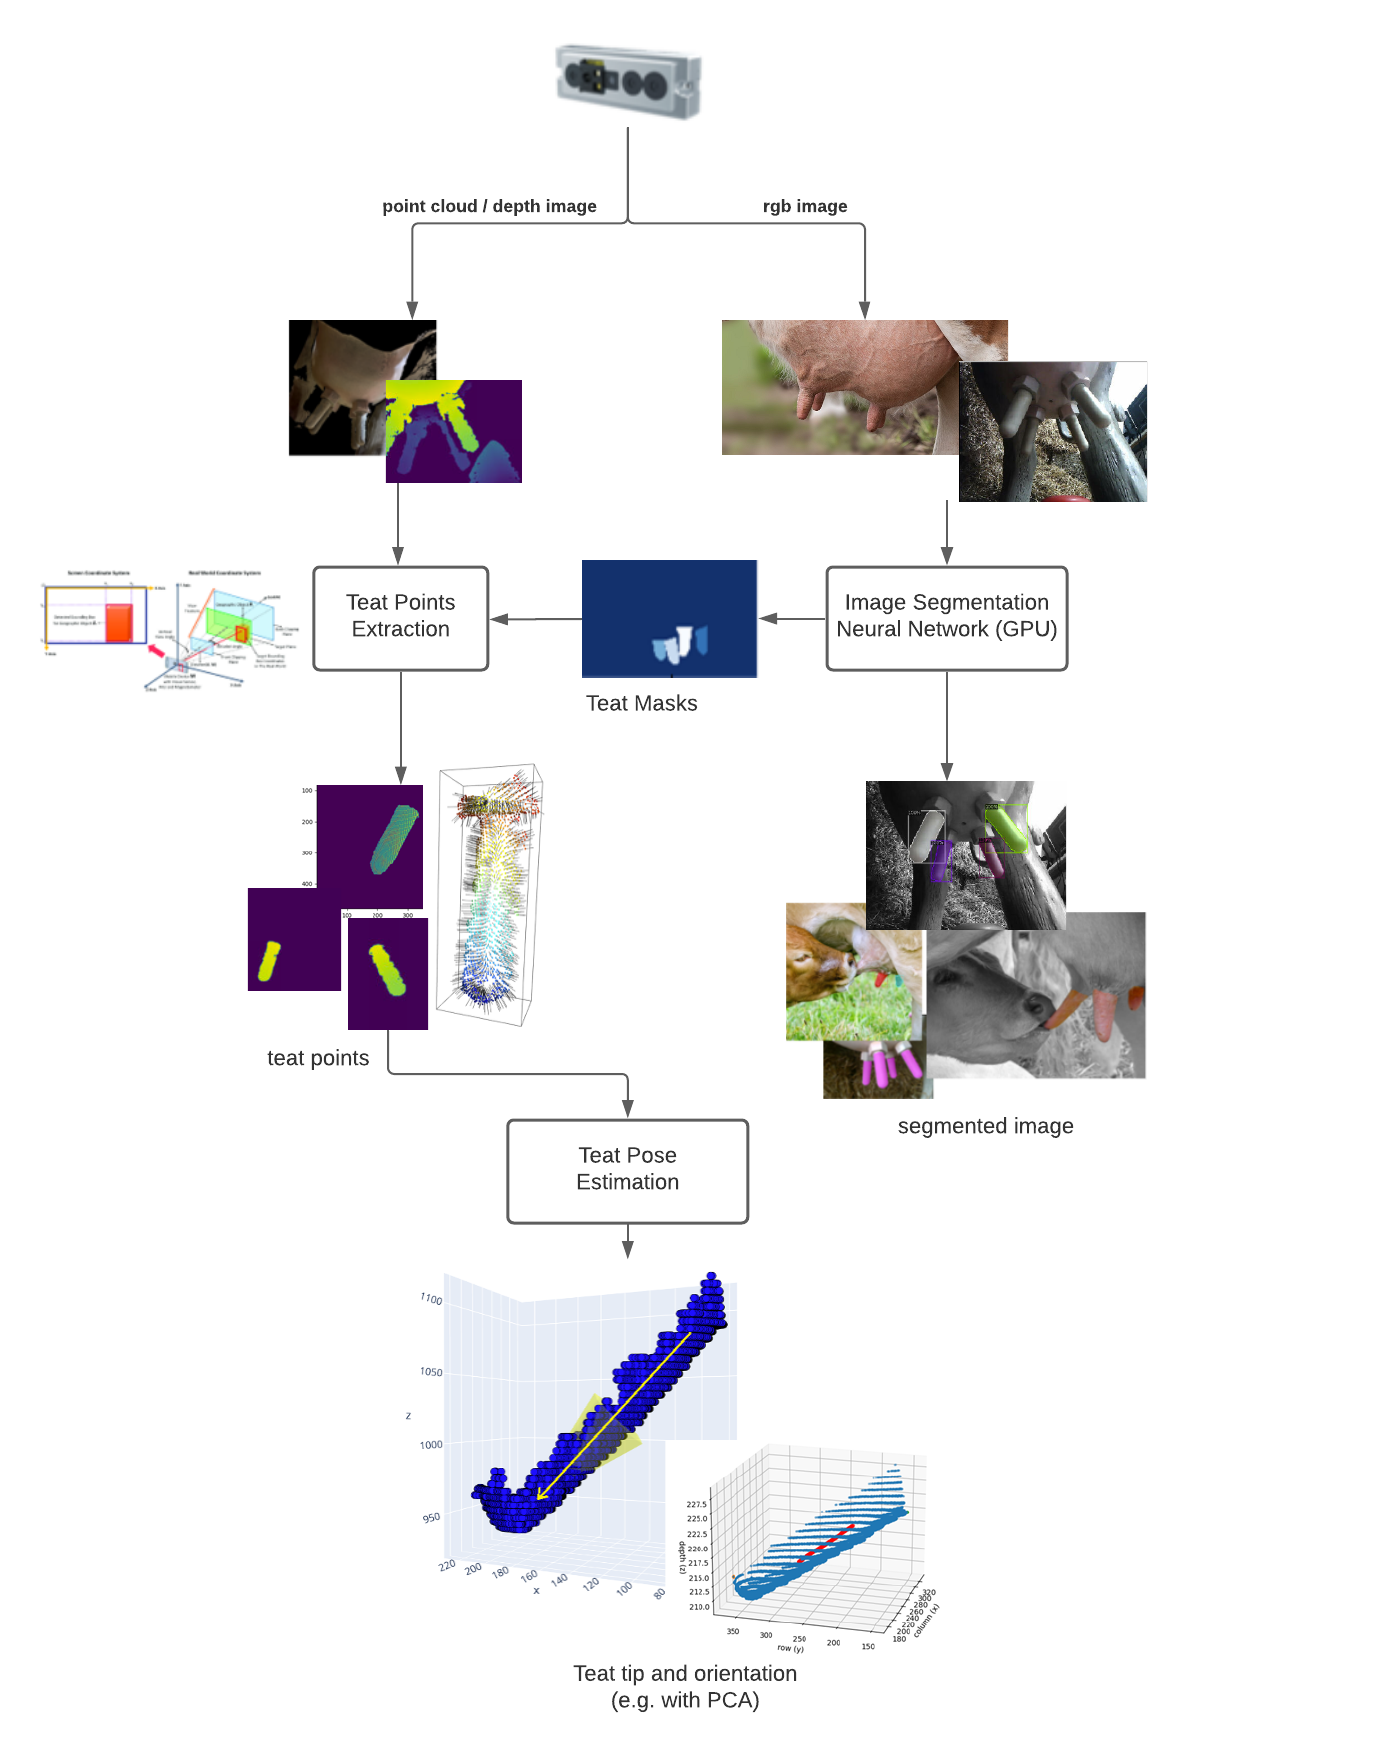
\includegraphics[width=1\textwidth]{images/cow_design.png}
    \caption{Pose Estimation Processing Pipeline Flowchart}
    \label{fig:cow_design}
\end{figure}

\newpage
\section{Camera Evaluation}
\label{appendix:camera_evaluation}

\begin{figure}[h]
        \centering
        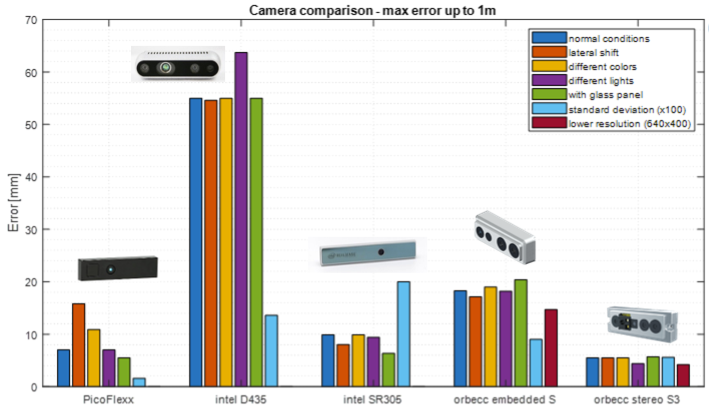
\includegraphics[width=0.8\textwidth]{images/camera_choice.png}
        \caption{Camera Performance Evaluation}
        \label{fig:camera_choice}
    \end{figure}
  
  
  
\newpage
\section{Pose Estimation Error Correlogram}  
\label{appendix:correlogram}
\begin{figure}[h]
        \centering
        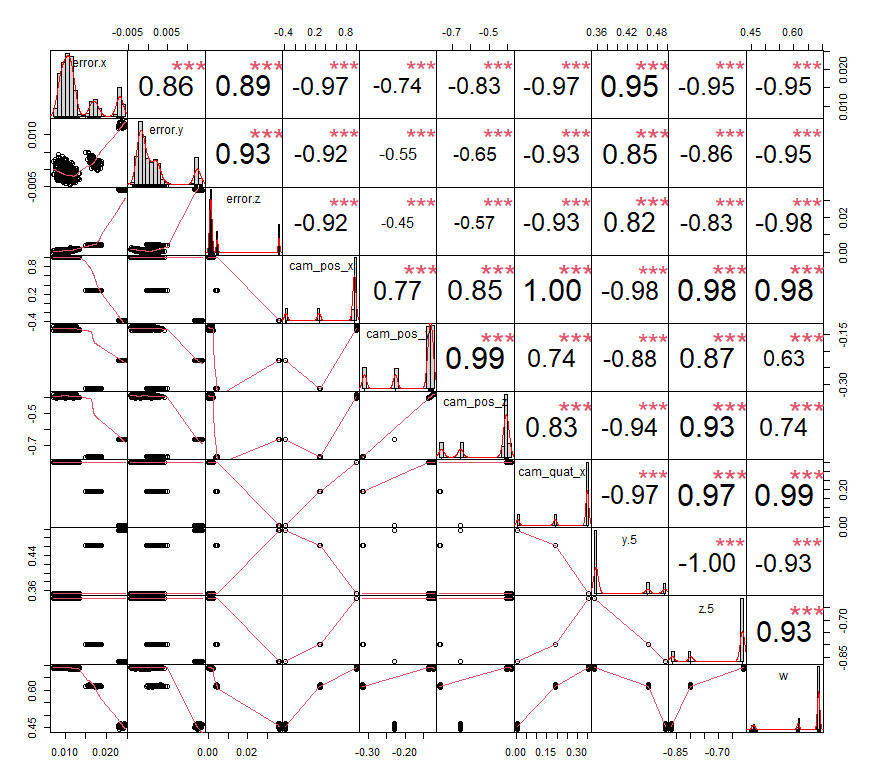
\includegraphics[width=0.9\textwidth]{images/r_correlogram.png}
        \caption{Correlogram of the errors in (x, y, z) and the camera position variables (x, y, z, quaternion) for the MAV algorithm.}
        \label{fig:correlogram}
\end{figure}


\end{document}

